\documentclass[12pt]{article}

\usepackage{amsmath,amstext,amssymb,graphicx,graphics,color}

%%%%%%%%%%%%%%%%%%%% Format  %%%%%%%%%%%%%%%%%%%%
\addtolength{\hoffset}{-.6cm}
\addtolength{\textwidth}{1.2cm}
\addtolength{\voffset}{-.5cm}
\addtolength{\textheight}{1.5cm}

%%%%%%%%%%%%%%%%%%%% Headings  %%%%%%%%%%%%%%%%%%%%
\usepackage{fancyhdr}
\pagestyle{fancy}
\renewcommand{\sectionmark}[1]{\markright{\thesection\ #1}}
\fancyhf{} \fancyhead[LE,RO]{\bfseries\thepage} \fancyhead[LO]{\bfseries\rightmark}
\fancyhead[RE]{\bfseries\leftmark}
\renewcommand{\headrulewidth}{0.5pt}
\renewcommand{\footrulewidth}{0pt}
\addtolength{\headheight}{0.5pt} \fancypagestyle{plain}{
  \fancyhead{}
  \renewcommand{\headrulewidth}{0pt}
}

% added 
\usepackage{listings, xcolor, float, dirtree, amsmath}
\usepackage{url}
\usepackage{hyperref}
\usepackage{graphicx}




% Define custom colors
\definecolor{codegreen}{rgb}{0,0.6,0}
\definecolor{codegray}{rgb}{0.5,0.5,0.5}
\definecolor{codepurple}{rgb}{0.58,0,0.82}
\definecolor{backcolour}{rgb}{0.95,0.95,0.92}

% Setup the listings environment
\lstset{
    backgroundcolor=\color{backcolour},  
    commentstyle=\color{codegreen},
    keywordstyle=\color{magenta},
    numberstyle=\tiny\color{codegray},
    stringstyle=\color{codepurple},
    basicstyle=\footnotesize\ttfamily, % or \small or \scriptsize etc.
    breakatwhitespace=false,         
    breaklines=true,                 
    captionpos=b,                    
    keepspaces=true,                 
    numbers=left,                    
    numbersep=5pt,                  
    showspaces=false,                
    showstringspaces=false,
    showtabs=false,                  
    tabsize=2
}

\title{Crystallography Peak Detection at CXLS}
\author{Eric Everett and Adam Kurth}

\begin{document}

\maketitle

\begin{abstract}

This paper explores the application of deep learning techniques at Arizona State University's (ASU) Compact X-ray Light Source (CXLS) to analyze experimental data from various modalities, primarily focusing on X-ray crystallography using the Dectris Eiger 4M detector. Traditional methods of predicting photon energy and sample-detector distance are challenged by dynamic scattering, intrinsic noise, and the CXLS low flux X-ray beam, prompting the need for more advanced solutions. Utilizing the CrystFEL\cite{crystfel} software, we simulate diffraction images for protein 1IC6.pdb across a matrix of nine variable combinations involving photon energies and camera length. Our approach employs convolutional neural networks (CNNs), testing various architectures for binary classification of peak detection and prediction of experimental parameters. The scope of this research wishes to further expand this with modifications in the architecture to accommodate for spectroscopy data, although this is beyond the extent of this manuscript. By integrating different experimental conditions, we anticipate broader applications and improved experimental outcomes.

\end{abstract}

\section{Introduction}

\subsection{ASU CXFEL Labs}

At Arizona State University (ASU), we are at the forefront of developing the world's first Compact X-ray Light Source (CXLS), a scaled-down 10 meter version of the traditionally large X-ray Free-Electron Lasers (XFELs), which typically extend over a kilometer. This revolutionary device emits X-ray pulses at the femtosecond scale and operates at a kilohertz frequency. These X-rays are used to scatter off of a sample where we can collect scatting images and collect data on these samples. Because of the nature of this X-ray beam, samples receive low radiation damage and high resolution scattering images can be collected.

\begin{figure}
    \centering
    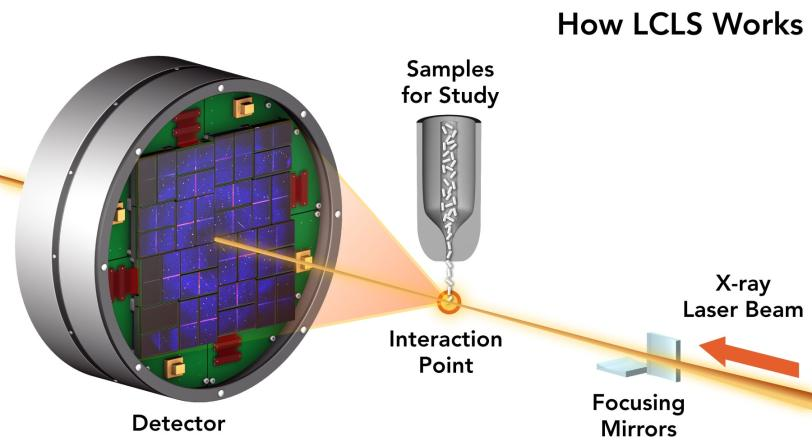
\includegraphics[width=0.5\textwidth]{lcls}
    \caption{This is an example of the X-ray beam interacting with a sample and the diffraction pattern being detected. This specific illustration is from the Linear Accelerator Coherent Light Source (LCLS). \cite{lcls_diagram}}
    \label{fig:lcls}
\end{figure}

The ability to scale down our X-ray light source comes from our techniques to generate X-rays. Other sources are so long in part due to the use of magnetic undulator to cause X-ray emission from relativistic electrons. At ASU we align our relativistic electron beam with a high power IR laser in space and time, generating X-rays from a process called Inverse Compton Scattering. The compact nature of the CXLS results in significant cost reductions, making these machines more viable for construction at other facilities. This will push research in fields like material science and pharmaceuticals that greatly benefit from having X-ray light sources for research.

Central to the functionality of the CXLS is the Dectris Eiger 4M detector, known for its high resolution and sensitivity for X-ray detection, which are crucial for capturing intricate diffraction patterns from protein crystals. However, the analysis of these patterns is complex and often labor-intensive, necessitating manual corrections to address data inaccuracies. Additionally, the CXLS has a low flux X-ray beam compared to other XFEL's, which complicates peak detection in both crystallography and spectroscopy images. The presence of scattering noise, largely due to the water content within protein samples, further complicates analyses. These challenges underscore the need for developing advanced methodologies that improve both the precision and efficiency of data processing at the CXLS.

\subsection{Project Outline}

The goal is this project is to lay the foundations for developing data analysis techniques for the CXLS using deep neural networks. Due to the CXLS still being in the preparation phase for experiments, we will be simulating diffraction data to train our models. This diffraction data is the resulting Bragg peaks from the experiment. In crystallography, Bragg peaks are the result from the constructive interference of X-rays scattered by the planes of atoms in a crystalline lattice, and they are crucial for determining the crystal structure of materials. Bragg peaks are defined by the following relationship, Bragg's law.

\begin{equation}
    n\lambda = 2d\sin(\theta)
\end{equation}

Where n is the order of the diffracted wave, $\lambda$ is the wavelength of the X-rays, d is the spacing between the crystal planes in the material, and $\theta$ is the angle at which the X-rays strike the crystal planes.

For our simulations, we use the protein designated as 1IC6.pdb, sourced from the RCSB Protein Data Bank \cite{rcsb}. According to the RCSB Protein Data Bank, the \textit{proteinase K from Tritirachium album limber} is characterized by a resolution of 0.98 $\textup{~\AA}$. This enzyme is part of the tetragonal crystal system and belongs to the space group $P 4_3 2_1 2$\cite{rcsb}. The unit cell dimensions are defined as $a = b = 58.3$ $\textup{~\AA}$, $c = 63.6$ $\textup{~\AA}$, with the point group being $4/mmm$, or $422$ \cite{rcsb}. This detailed structural information is fundamental to our analysis and facilitates a more precise understanding of the protein's diffraction patterns. Below is a visual representation of the tetragonal crystal system\cite{tetragonal}.

\begin{figure}[H]
    \centering
    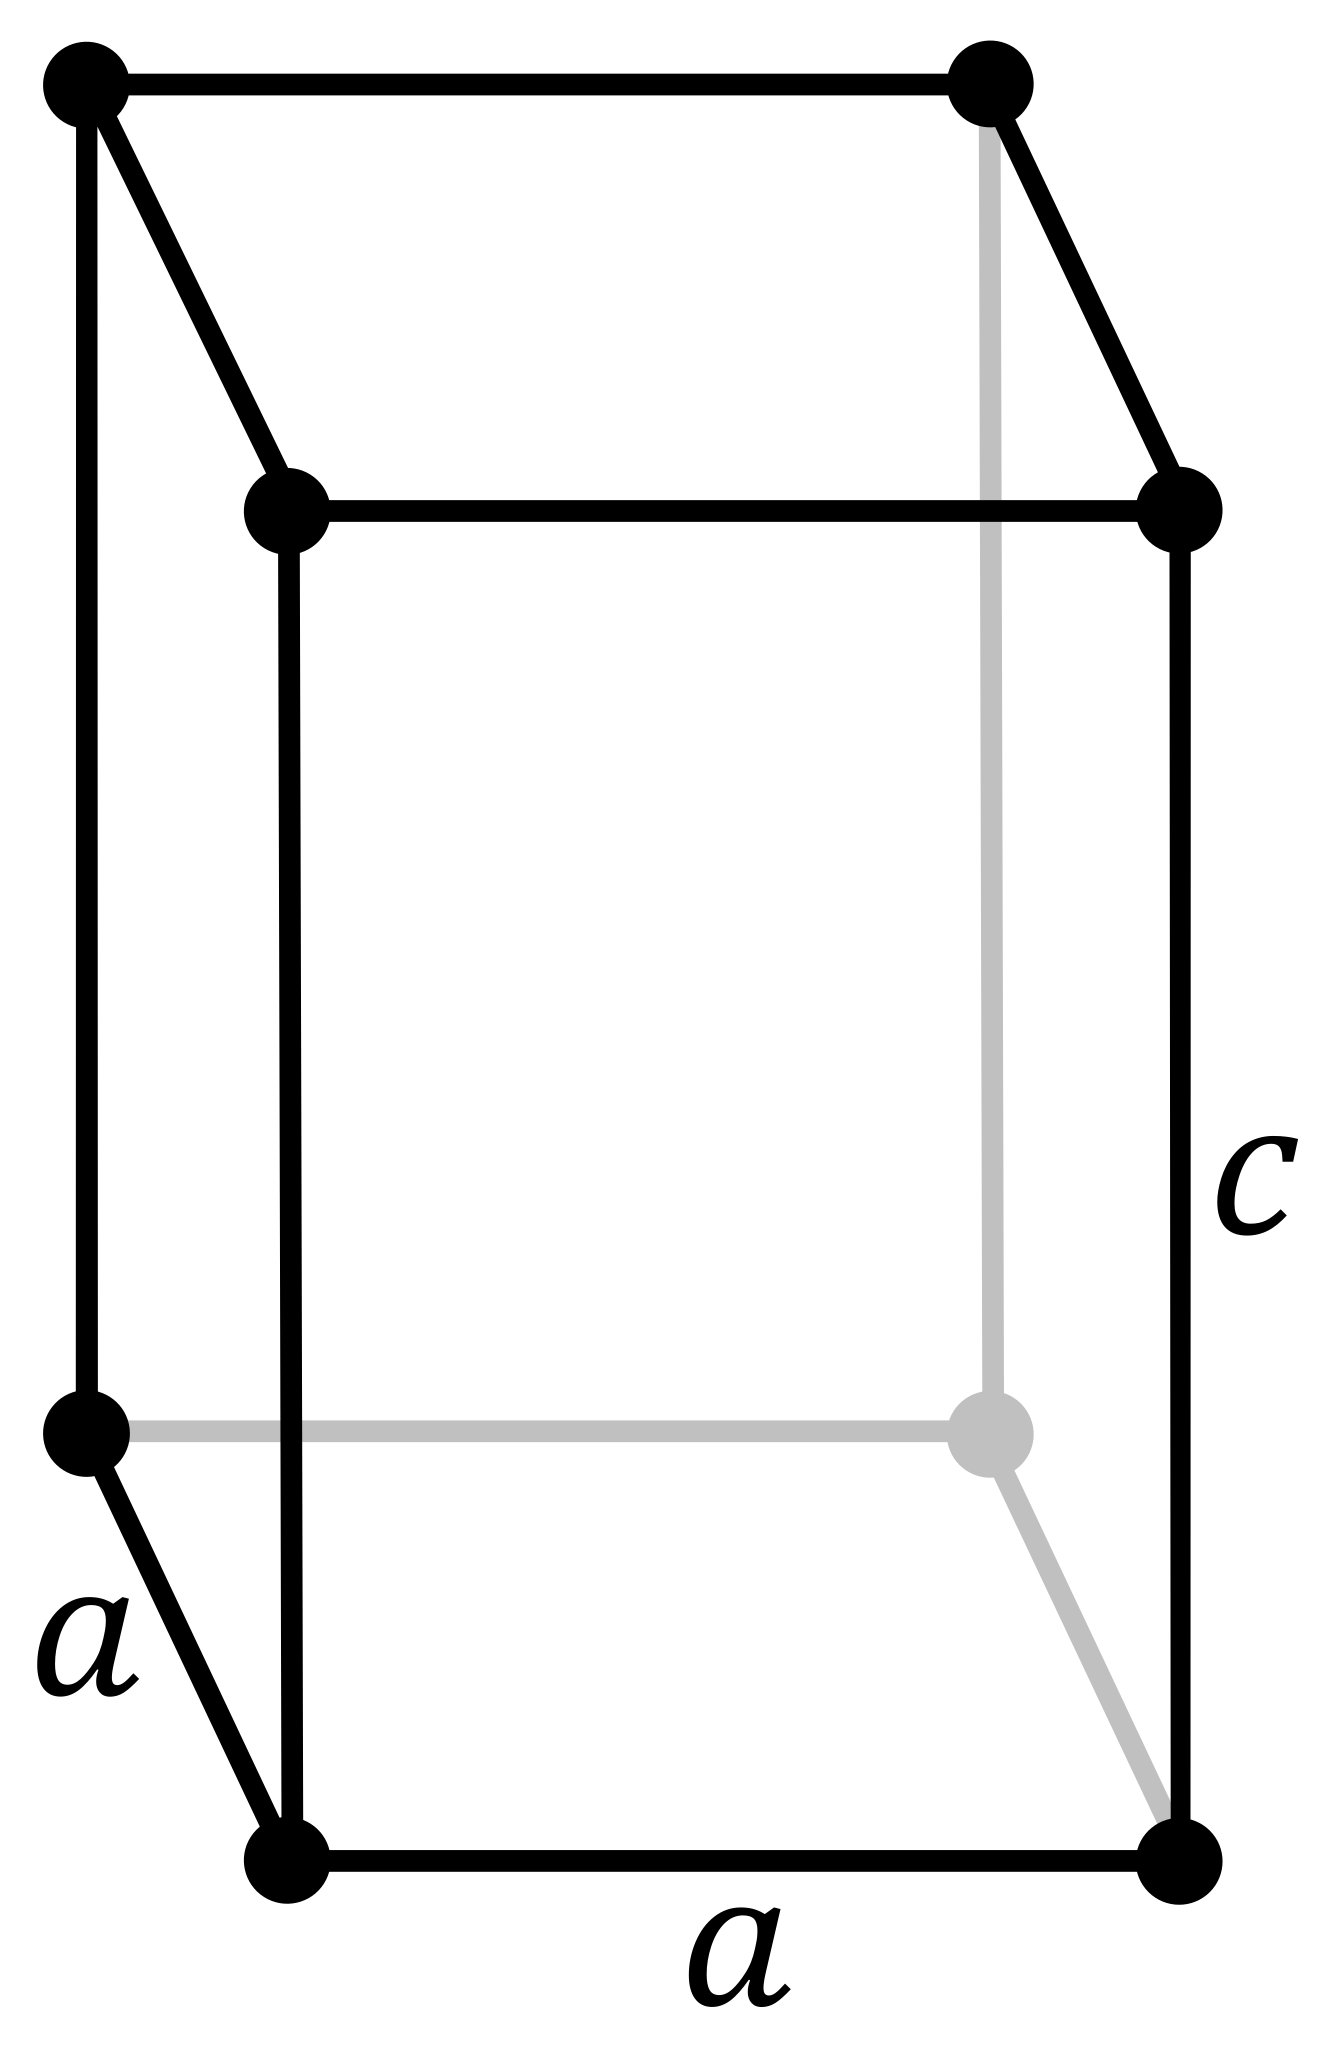
\includegraphics[scale=0.08]{tetragonal.png}
    \caption{Tetragonal Crystal System.}
    \label{fig:tetragonal}
\end{figure}

Using the X-ray diffraction images, we want to be able to determine attributes of 1IC6.pdb. However, before we can do that, we need to use these images to determine attributes of the experimental system. The three attributes we want to determine in this project from our detraction data is are there Bragg peaks present or is it just noise, what the incident photon energy is, and what the camera length is. In addition, we want to be able to detect where Bragg peaks are located. Due to the low photon flux from CXLS, especially compared to other X-ray light sources, the scattered Bragg peaks will appear much closer to the noise in the image, caused by water present in the proteins.

The incident photon energy greatly changes the diffraction data because of the relationship between the wavelength of the incident light and its energy. We can describe this relationship by a form of the Plank-Einstein relation.

\begin{equation}
    E = \frac{\hbar\ c}{\lambda}
\end{equation}

Where \(E\) is the energy, \(\hbar\) is Planck's constant, \(c\) is the speed of light, and $\lambda$ is the wavelength. We can see the dependence on $\lambda$ between the relationship with energy and with Bragg Law.

The camera length is another factor that will greatly change the diffraction data. As the camera length grows, there will be an increase angular spread from the scattered X-rays. An increased camera length can increase the spacial resolution of the data by spreading the signal over a greater area, however, this will also result in a weaker signal. Understanding these two parameters is a critical first step for data analysis. 

% CITE SOURCES!!! ^^^^^

\section{Methods}

\subsection{Data Simulation}

To contextualize the methodology employed in our simulations, it is pertinent to discuss the data format utilized—HDF5 (Hierarchical Data Format version 5) \cite{lochdf5}. This format is particularly favored in the field of crystallography for its capability to efficiently handle and store large datasets, such as those typically generated during crystallographic experiments \cite{hdf5}. One of the notable features of HDF5 is its support for storing a flexible number of individual snapshots within a single file \cite{hdf5}. This capability is essential for capturing multiple images under varying experimental conditions without the need to switch files, significantly streamlining the analysis process \cite{hdf5}.

Moreover, HDF5 files facilitate the clear visualization of Bragg peaks within these snapshots. Bragg peaks are crucial for determining the atomic structure of crystals, as they reflect the positions and intensities of diffracted X-rays. The ability to observe and analyze these peaks across various snapshots enhances our capacity to discern changes and similarities in crystal structures under different experimental conditions. The attributes of HDF5 make it an exemplary choice for crystallography, where precision, efficiency, and meticulous data management are paramount.

Following the selection of the appropriate data format, we proceeded to simulate the diffraction patterns using the \texttt{pattern\_sim} module of the CrystFEL software suite \cite{crystfel_patternsim}. These simulations are designed to closely replicate the scattering patterns characteristic of real experimental data, providing a solid foundation for training our deep learning models. An example of the configuration script used for our simulations is depicted in Figure~\ref{fig:lcls}, illustrating the setup and parameters that guide our simulation process. This strategic approach not only ensures the accuracy of our simulations but also enhances the effectiveness of the subsequent analysis performed by our deep learning models.

\begin{figure}[H]
\centering
\begin{lstlisting}[language=bash]
#!/bin/bash

# Global configurations
NAME="$1"                              # Experiment or job prefix
TASKS="$2"                             # Number of tasks to request for each job
PHOTON_ENERGY="$"6000                  # Photon energy input
# ...
# pattern_sim specifications
GEOM="Eiger4M.geom"                    # Geometry file
CRYSTAL="1IC6.cell"                    # Crystal file
INPUT="1IC6.pdb.hkl"                   # Constant HKL input file
POINT_GROUP="4/mmm"
CRYSTAL_SIZE_MIN=10000
CRYSTAL_SIZE_MAX=10000
SPECTRUM="tophat"
SAMPLING=7
BANDWIDTH=0.01
N_PHOTONS=3e8
BEAM_RADIUS=5e-6
NUMBER_OF_PATTERNS=10000
# ...
\end{lstlisting}
\caption{Example of BASH script used with \texttt{pattern\_sim} \cite{crystfel_patternsim} to simulate diffraction data.}
\label{fig:bashSubmitionExample}
\end{figure}

The first fixed parameters in our simulation are the detector geometry of the Dectris Eiger 4M, which produces a 2069$\times$2163 image. Additionally, we have fixed parameters for the protein and its 10 micro crystal environment, as well as for the incident X-ray beam, including photon flux and beam radius. We create 9 total datasets of simulated data by varying the previously mention parameters photon energy and camera length. Table~\ref{tab:dataset-parameters} below outlines these datasets.

\begin{table}[H]
\centering
\caption{Datasets generated by varying camera length and photon energy.}
\label{tab:dataset-parameters}
\begin{tabular}{c|c|c}
Dataset & Camera Length (m) & Photon Energy (keV) \\
\hline
01 & 0.15 & 6 \\
02 & 0.15 & 7 \\
03 & 0.15 & 8 \\
04 & 0.25 & 6 \\
05 & 0.25 & 7 \\
06 & 0.25 & 8 \\
07 & 0.35 & 6 \\
08 & 0.35 & 7 \\
09 & 0.35 & 8 \\
\end{tabular}
\end{table}

All of the resulting images from pattern\_sim are pure signal from the diffraction simulations, and will call these \textit{peak} images.

To create the realistic dataset, we must generate the water background images which introduce noise to each respective dataset. These are the diffraction patterns caused by the water within the proteins that make analysis of Bragg peaks difficult. To simulate these water background images we use a software developed by Kirian Lab, \texttt{reborn}, which is a Python package for X-ray diffraction simulation and analysis under the Born approximation \cite{reborn}. Again, like with peak images, we use the Dectris Eiger 4M detector geometry, and very the incident photon energy and camera length. Unlike with peaks data, we only simulate 1 water background image for all 9 data sets. This is because we expect the water background noise to be fairly consistent from shot to shot. We will refer to these images as \textit{water-background} images.

As we see here, the photon energy is held constant at 6keV, while the camera length is 0.15m in Figure~\ref{fig:water1} and 0.35 in Figure~\ref{fig:water7}.

\begin{figure}[H]
    \centering
    % First image
    \begin{minipage}{0.49\textwidth}
        \centering
        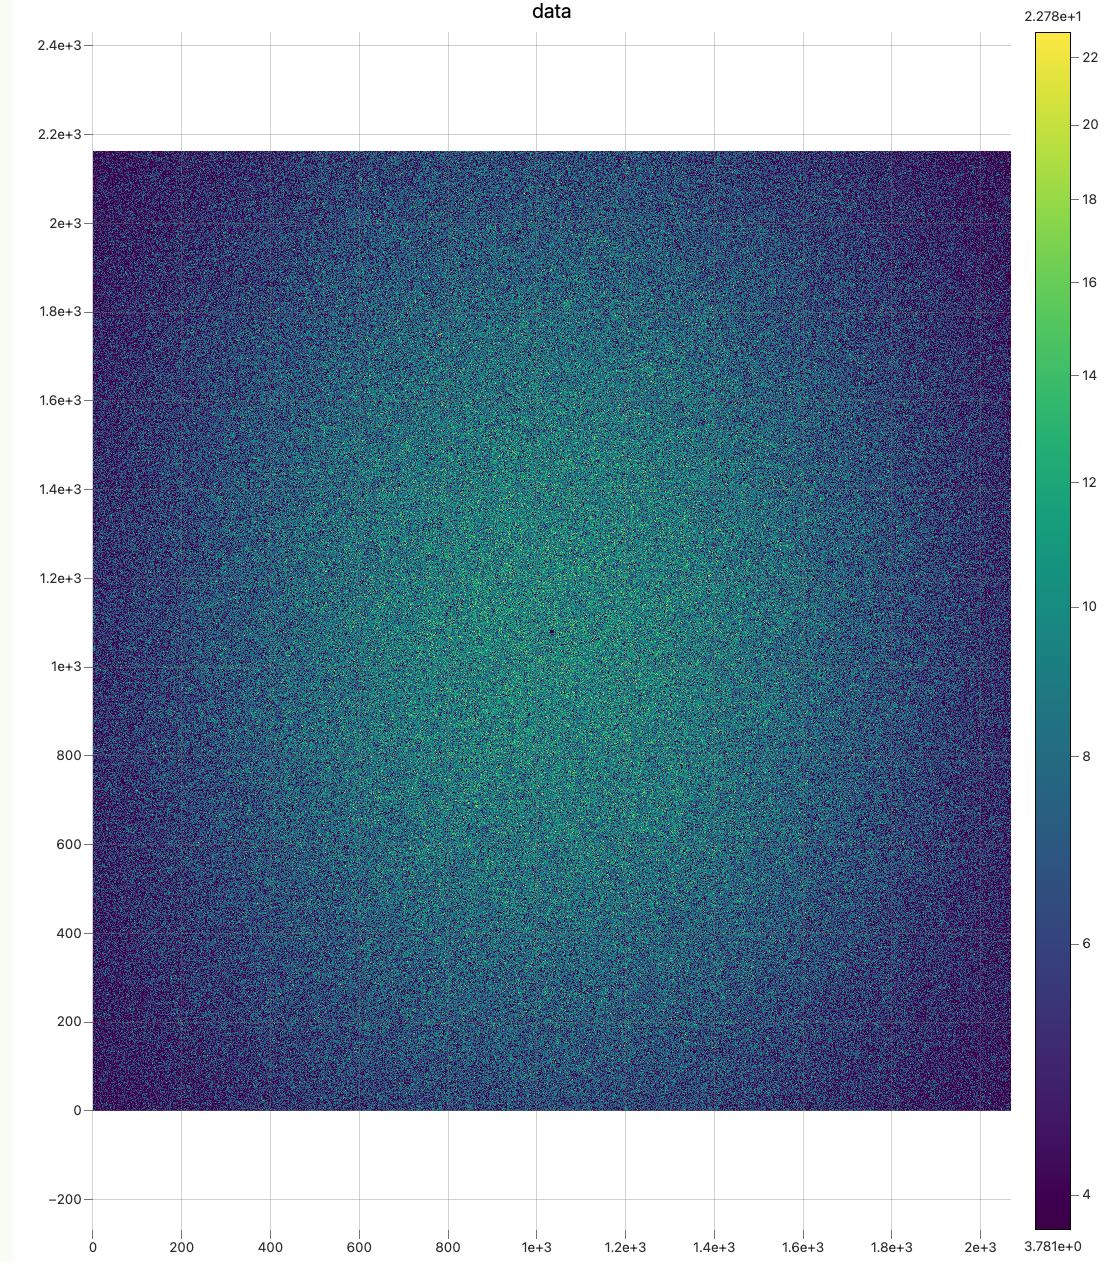
\includegraphics[width=\textwidth]{water01.png}
        \caption{Camera length of 0.15}
        \label{fig:water1}
    \end{minipage}
    \hfill
    % Second image
    \begin{minipage}{0.49\textwidth}
        \centering
        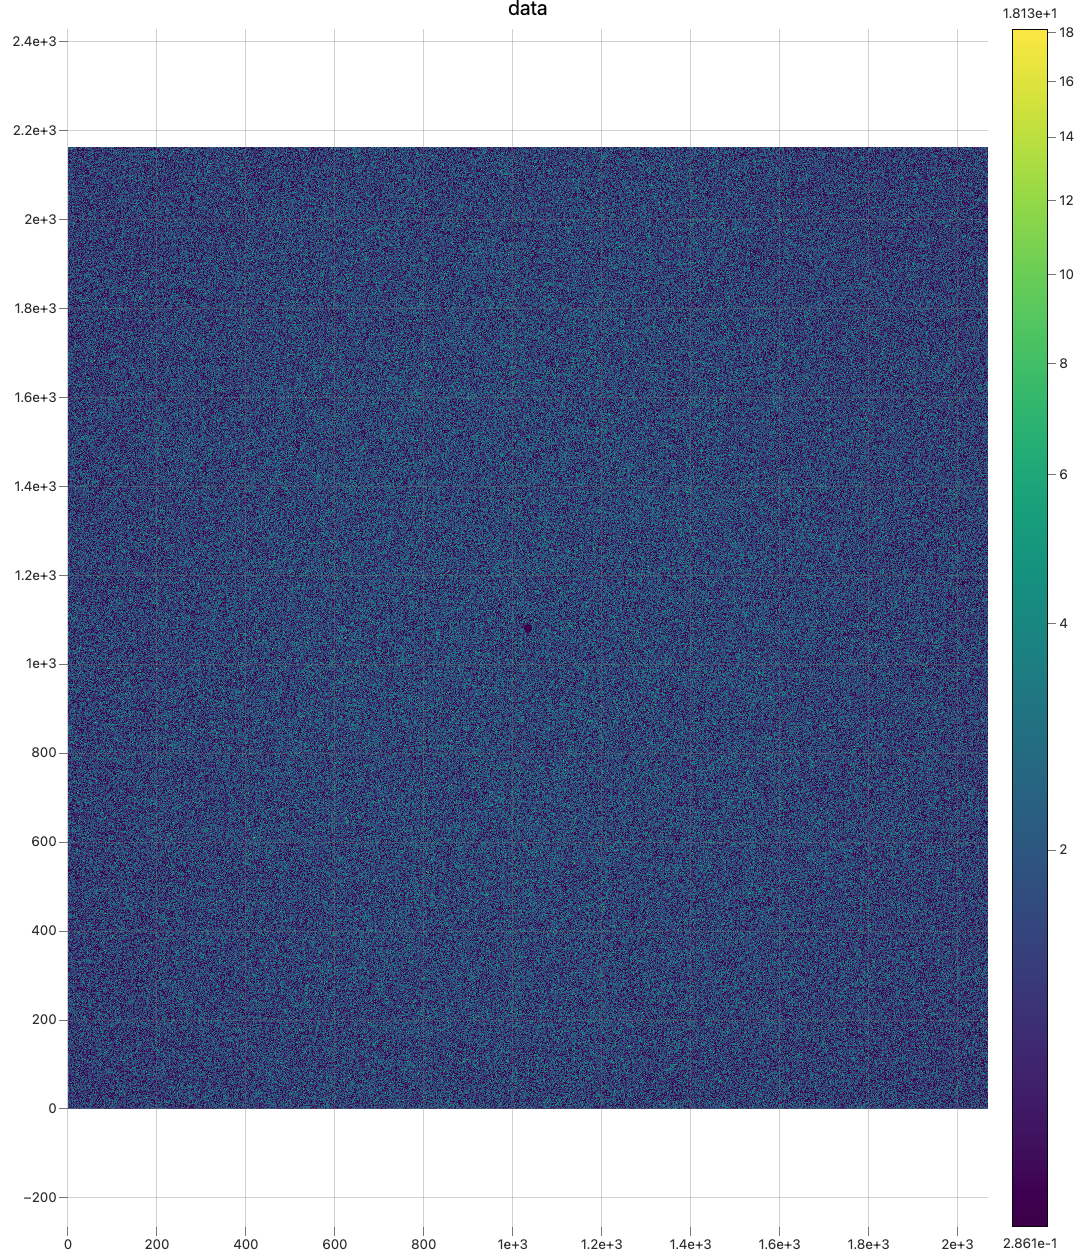
\includegraphics[width=\textwidth]{water07.png}
        \caption{Camera length of 0.35}
        \label{fig:water7}
    \end{minipage}
\end{figure}

To create the realistic noisy images from the simulated peak and water-background images. We simply overlayed the water-background images and peak images with the same parameter combination; that is, the same photon energy and camera length values. We will refer to these as \textit{overlay} images.

\subsection{Data Management}

In handling all of the generated images with different parameter combinations, file management was an important part of the development of this project. Figure~\ref{fig:dirtree} shows the base \texttt{images/} directory and the structure that is used for the organization of these images. Notably, the \texttt{labels} directory holds the binary heatmaps to predict Bragg peak location. Its purpose is to predict Bragg peaks upon testing. However, in the time frame of this project we did not have the time necessary to develop this feature, and it will be discuss later what we used for our labels for the different classification problems.\\

\begin{figure}[H]
\dirtree{%
.1 images/.
.2 peaks/.
.3 01/.
.4 01\_6keV\_clen01\_000001.h5.
.4 ....
.3 02/.
.4 02\_7keV\_clen01\_000001.h5.
.4 ....
.3 ....
.3 09/.
.4 09\_8keV\_clen03\_000001.h5.
.4 ....
.2 labels/.
.2 peaks\_water\_overlay/.
.2 water/.
}
\caption{Directory structure for images.} % Caption for the dirtree
\label{fig:dirtree} % Label for referencing
\end{figure}

Multiple Python scripts were developed to create a robust file management system. These files are \texttt{process\_directory.py} (Figure~\ref{fig:process_directory}), \texttt{process.py} (Figure~\ref{fig:process}), \texttt{path.py} (Figure~\ref{fig:path}), \texttt{data.py} (Figure~\ref{fig:data}). The development of a robust file management system is fundamental to this project, especially as it continues to scale with future development.\\

\begin{figure}[H]
    \centering
    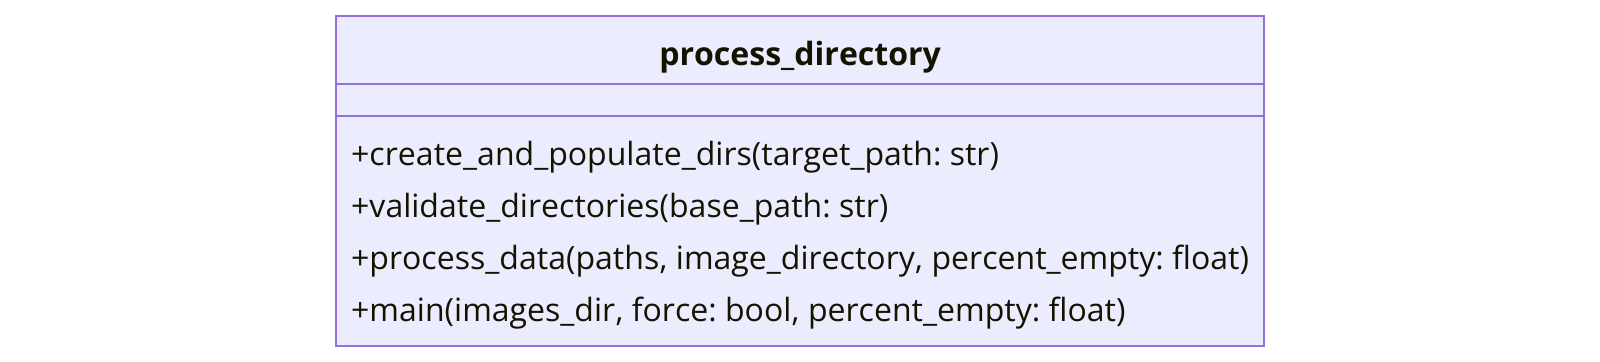
\includegraphics[width=0.8\textwidth]{uml_diagrams/process_directory_uml.png}
    \caption{process\_directory.py UML diagram}
    \label{fig:process_directory}
\end{figure}

Upon running \texttt{process\_directory.py}, the script calls classes from \texttt{process.py}, \texttt{path.py}. Namely, the \texttt{Processor} class which is responsible for generating the overlay images, and the \texttt{PathManager} class which keeps track of all the generated files, by selecting the datasets. But \texttt{process\_directory.py} takes the peaks data (\texttt{images/peaks}) and casting every pixel into a binary value (0 or 1) based on a threshold. It's important to note that since the peak images were only signal, this threshold was arbitrary because everything diffracted in the simulation were photons. The script then saves the labeled images in \texttt{images/labels} which will be used later after the scope of this course. This script also takes the water-background image (\texttt{images/water}) of the respective dataset, and adds the two matrices from the peak image and water-background image. These overlay images are saving in \texttt{mages/peaks\_water\_overlay}.\\

\begin{figure}[H]
    \centering
    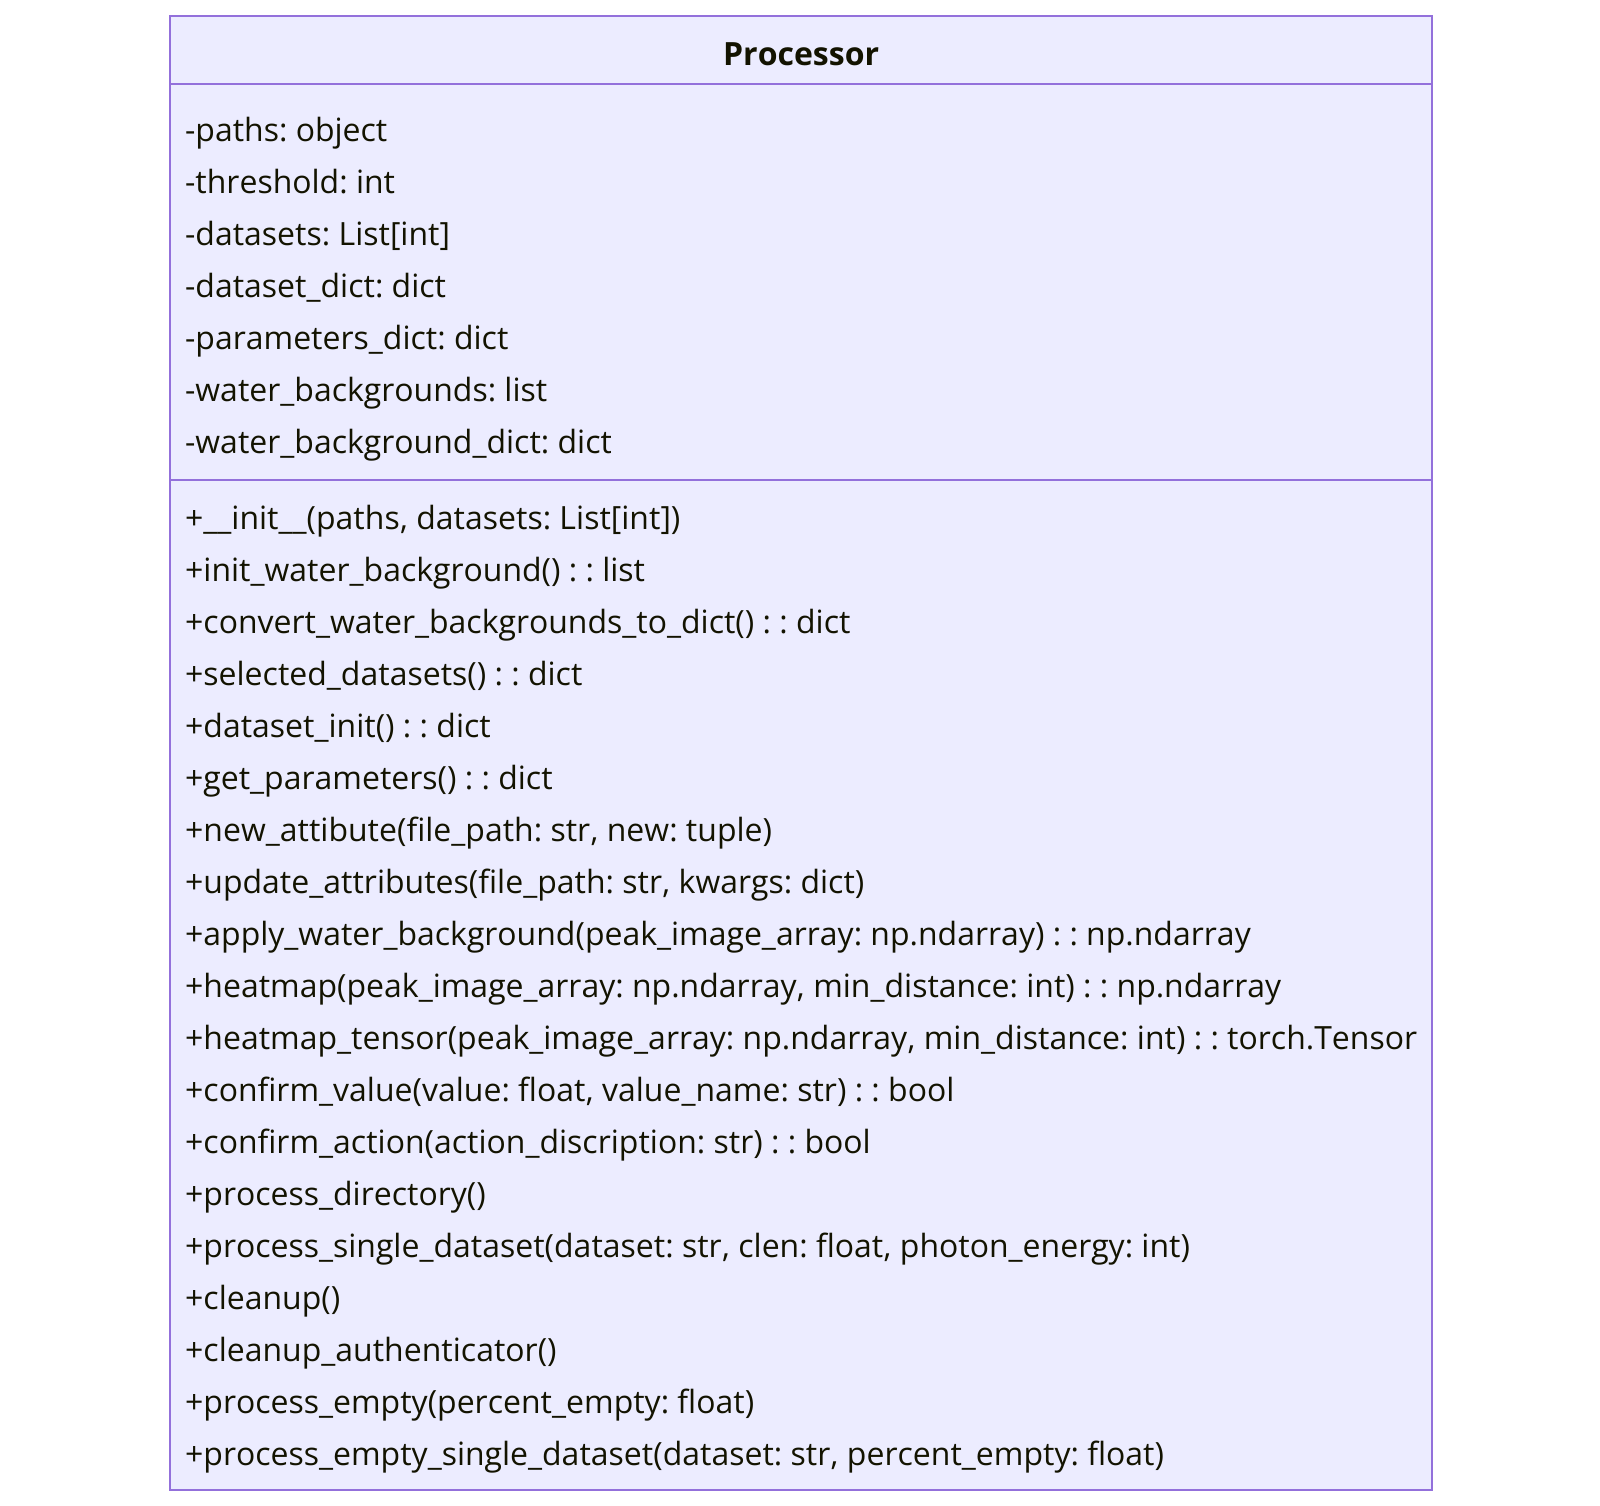
\includegraphics[width=0.6\textwidth]{uml_diagrams/process_uml.png}
    \caption{process.py UML diagram}
    \label{fig:process}
\end{figure}

With adequate training and testing in mind, the incorporation of "empty" images are necessary into the datasets. This is easily done by adding an argument that takes some input percent, say 50\% of the data in \texttt{images/peaks}, (say 50 images from the original 100) then adds that number of image back into the directories (to get 150). \texttt{images/peaks} and \texttt{images/labels} both will receive simply 0 matrices, \texttt{images/peak\_water\_overlay} will receive the water-background image of the respective dataset. Since we will be testing with the overlay images, its important for peak detection to distinguish between images with Bragg peaks, and without.\\

As mentioned the \texttt{Processor} class in \texttt{process.py}, works with \texttt{process\_directory.py}. In addition to generating new overlay images, and "empty" images, we also incorporate a validation check. This check ensures all the images have correct attributes assigned to them. This involves; the presence of Bragg peaks, the camera length, and photon energy. We prompt the user to select the datasets to be used for training and testing, in the \texttt{select\_datasets} function. This simply calls every dataset across the directories in \texttt{images/} and gets an updated number of images in each directory, and then calls the \texttt{get\_counts} function to count every selected directory. All of these steps in the script ensures homogeneous data to be used in training and testing.\\

\begin{figure}[H]
    \centering
    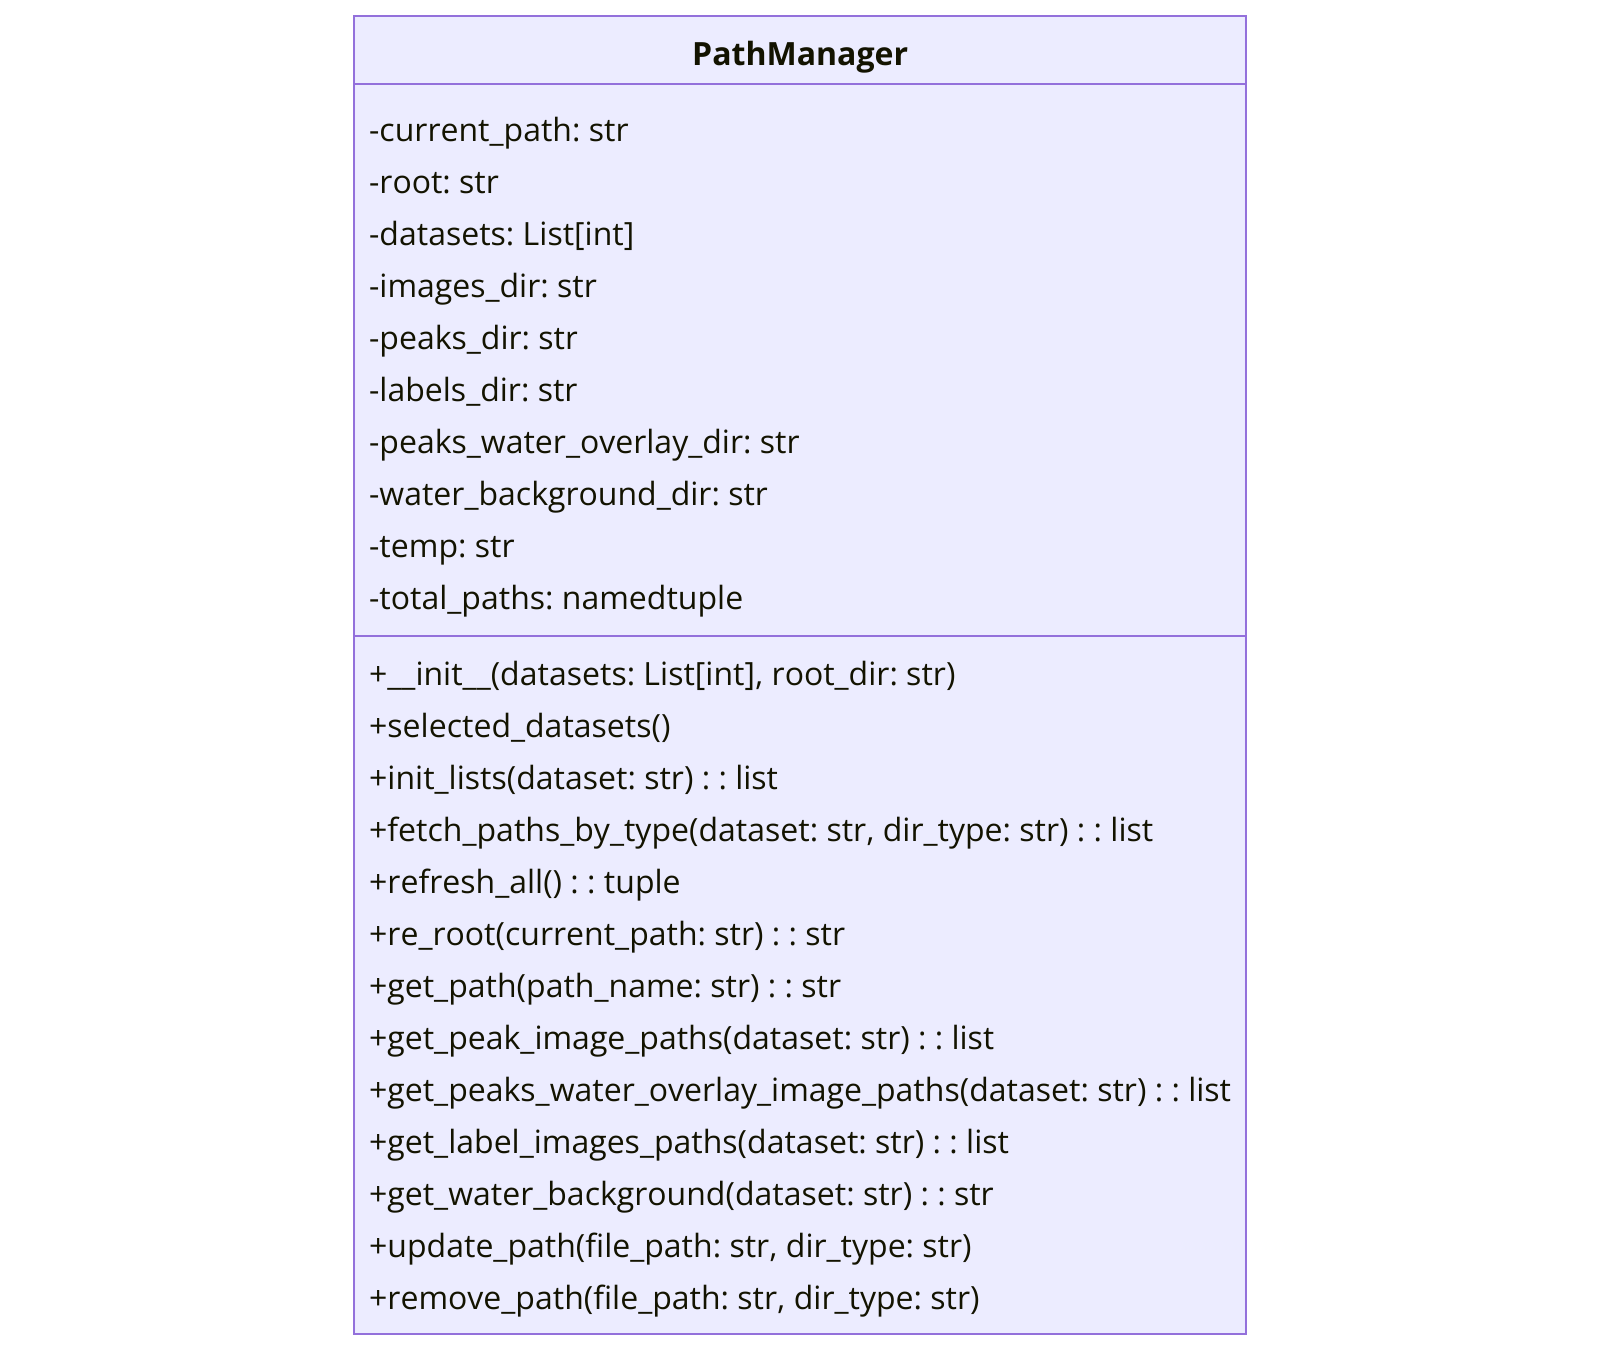
\includegraphics[width=0.7\textwidth]{uml_diagrams/path_uml.png}
    \caption{path.py UML diagram}
    \label{fig:path}
\end{figure}

The next step, is the load this into the PyTorch DataLoader. This functionality is incorporated in the class \texttt{DataManager} in \texttt{data.py}. This does the standard DataLoader instantiation from \texttt{torch.utils.datasets}, where the file paths from \texttt{PathManager} (therefore \texttt{images/}) are parsed according to their peak, overlay, and labels images. A partition of the data occurs where 80\% is used for training, and 20\% used for testing.\\

\begin{figure}[H]
    \centering
    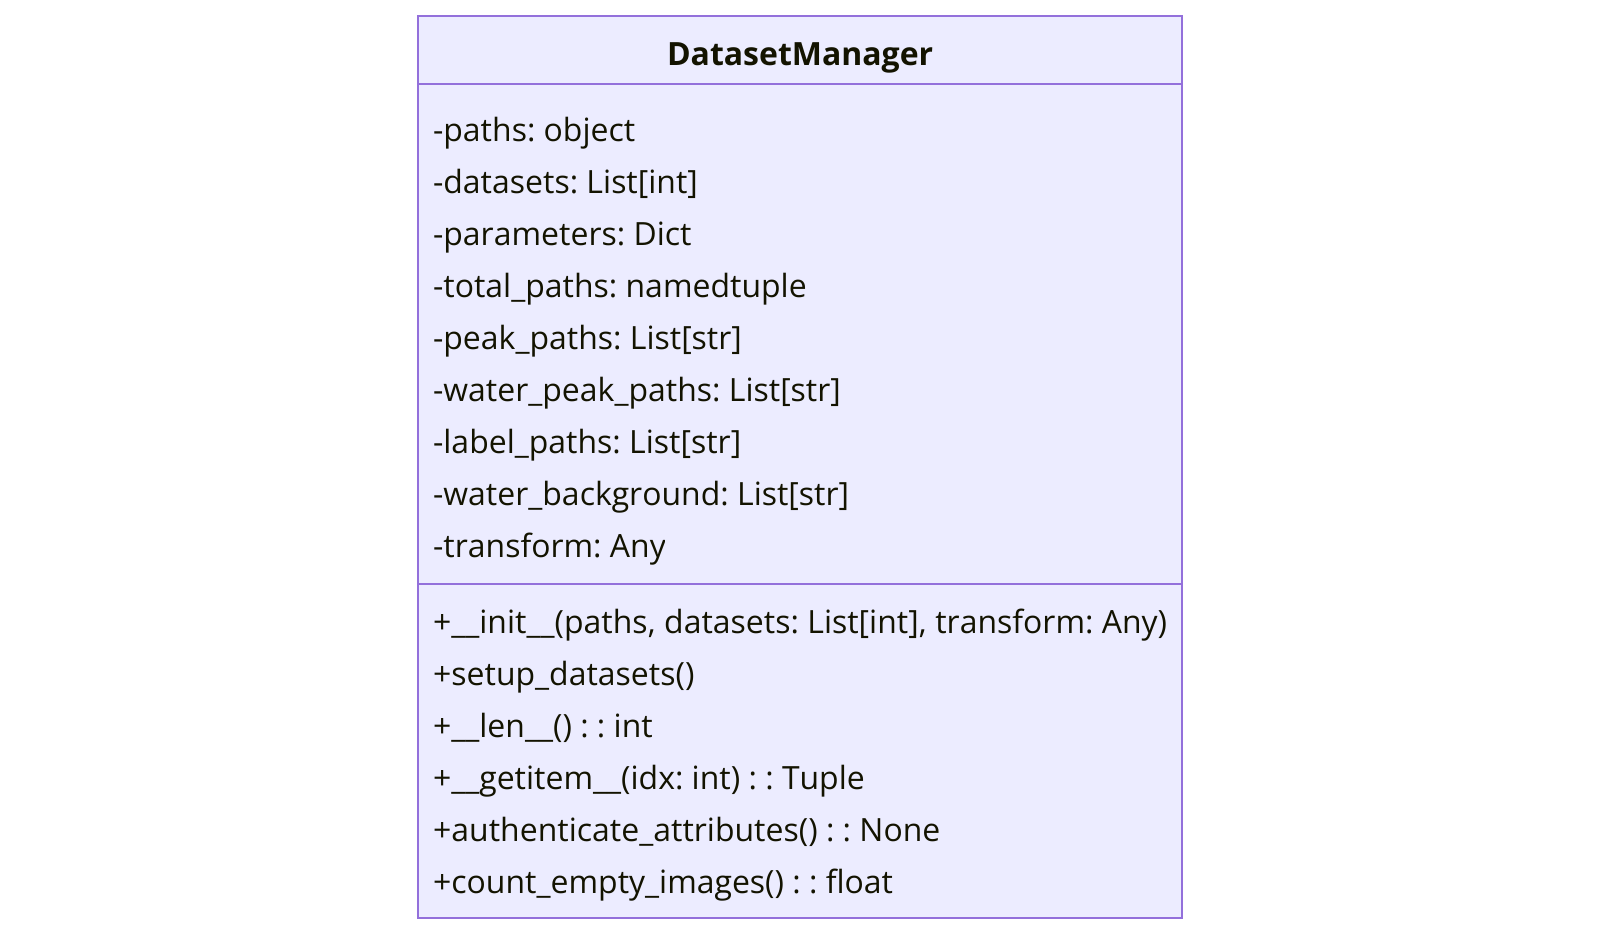
\includegraphics[width=0.75\textwidth]{uml_diagrams/data_uml.png}
    \caption{data.py UML diagram}
    \label{fig:data}
\end{figure}




\newpage
\subsection{Model Architectures}

As mention earlier, there are three parameters that we are looking to identify in each diffraction image, are Bragg peaks present, what is the incident photon energy, and what is the camera length. This can be defined as three-classification problem.  In addition, we want to be able to locate were Bragg peaks are in a diffraction image. Instead of building one large model that the give an output probability for every combination of the key parameters, three models are used for classification. This approach was agreed to be the best for further development, as these models are only functioning as initial test for classification with simulated data. We will later want to classify photon energy and camera length values more precisely and add models to find different parameters. Due to the nature of having multiple models, we implement a model pipeline for images to pass through to gather information. This will be elaborated on in the latter half of this section.\\

Each of these attributes we are classifying require different models, labels, optimizers, learning rates, loss functions, and other important parameters. To help keep concise and modular code we created classes in our \texttt{eval.py} file for each attribute to take advantage of Pythons object oriented capabilities. This helped the code greatly by only needing to instantiate an attribute we want to classify and pass the object around to relevant code like the training loop, evaluation, and the model pipeline.\\

\begin{figure}[H]
    \centering
    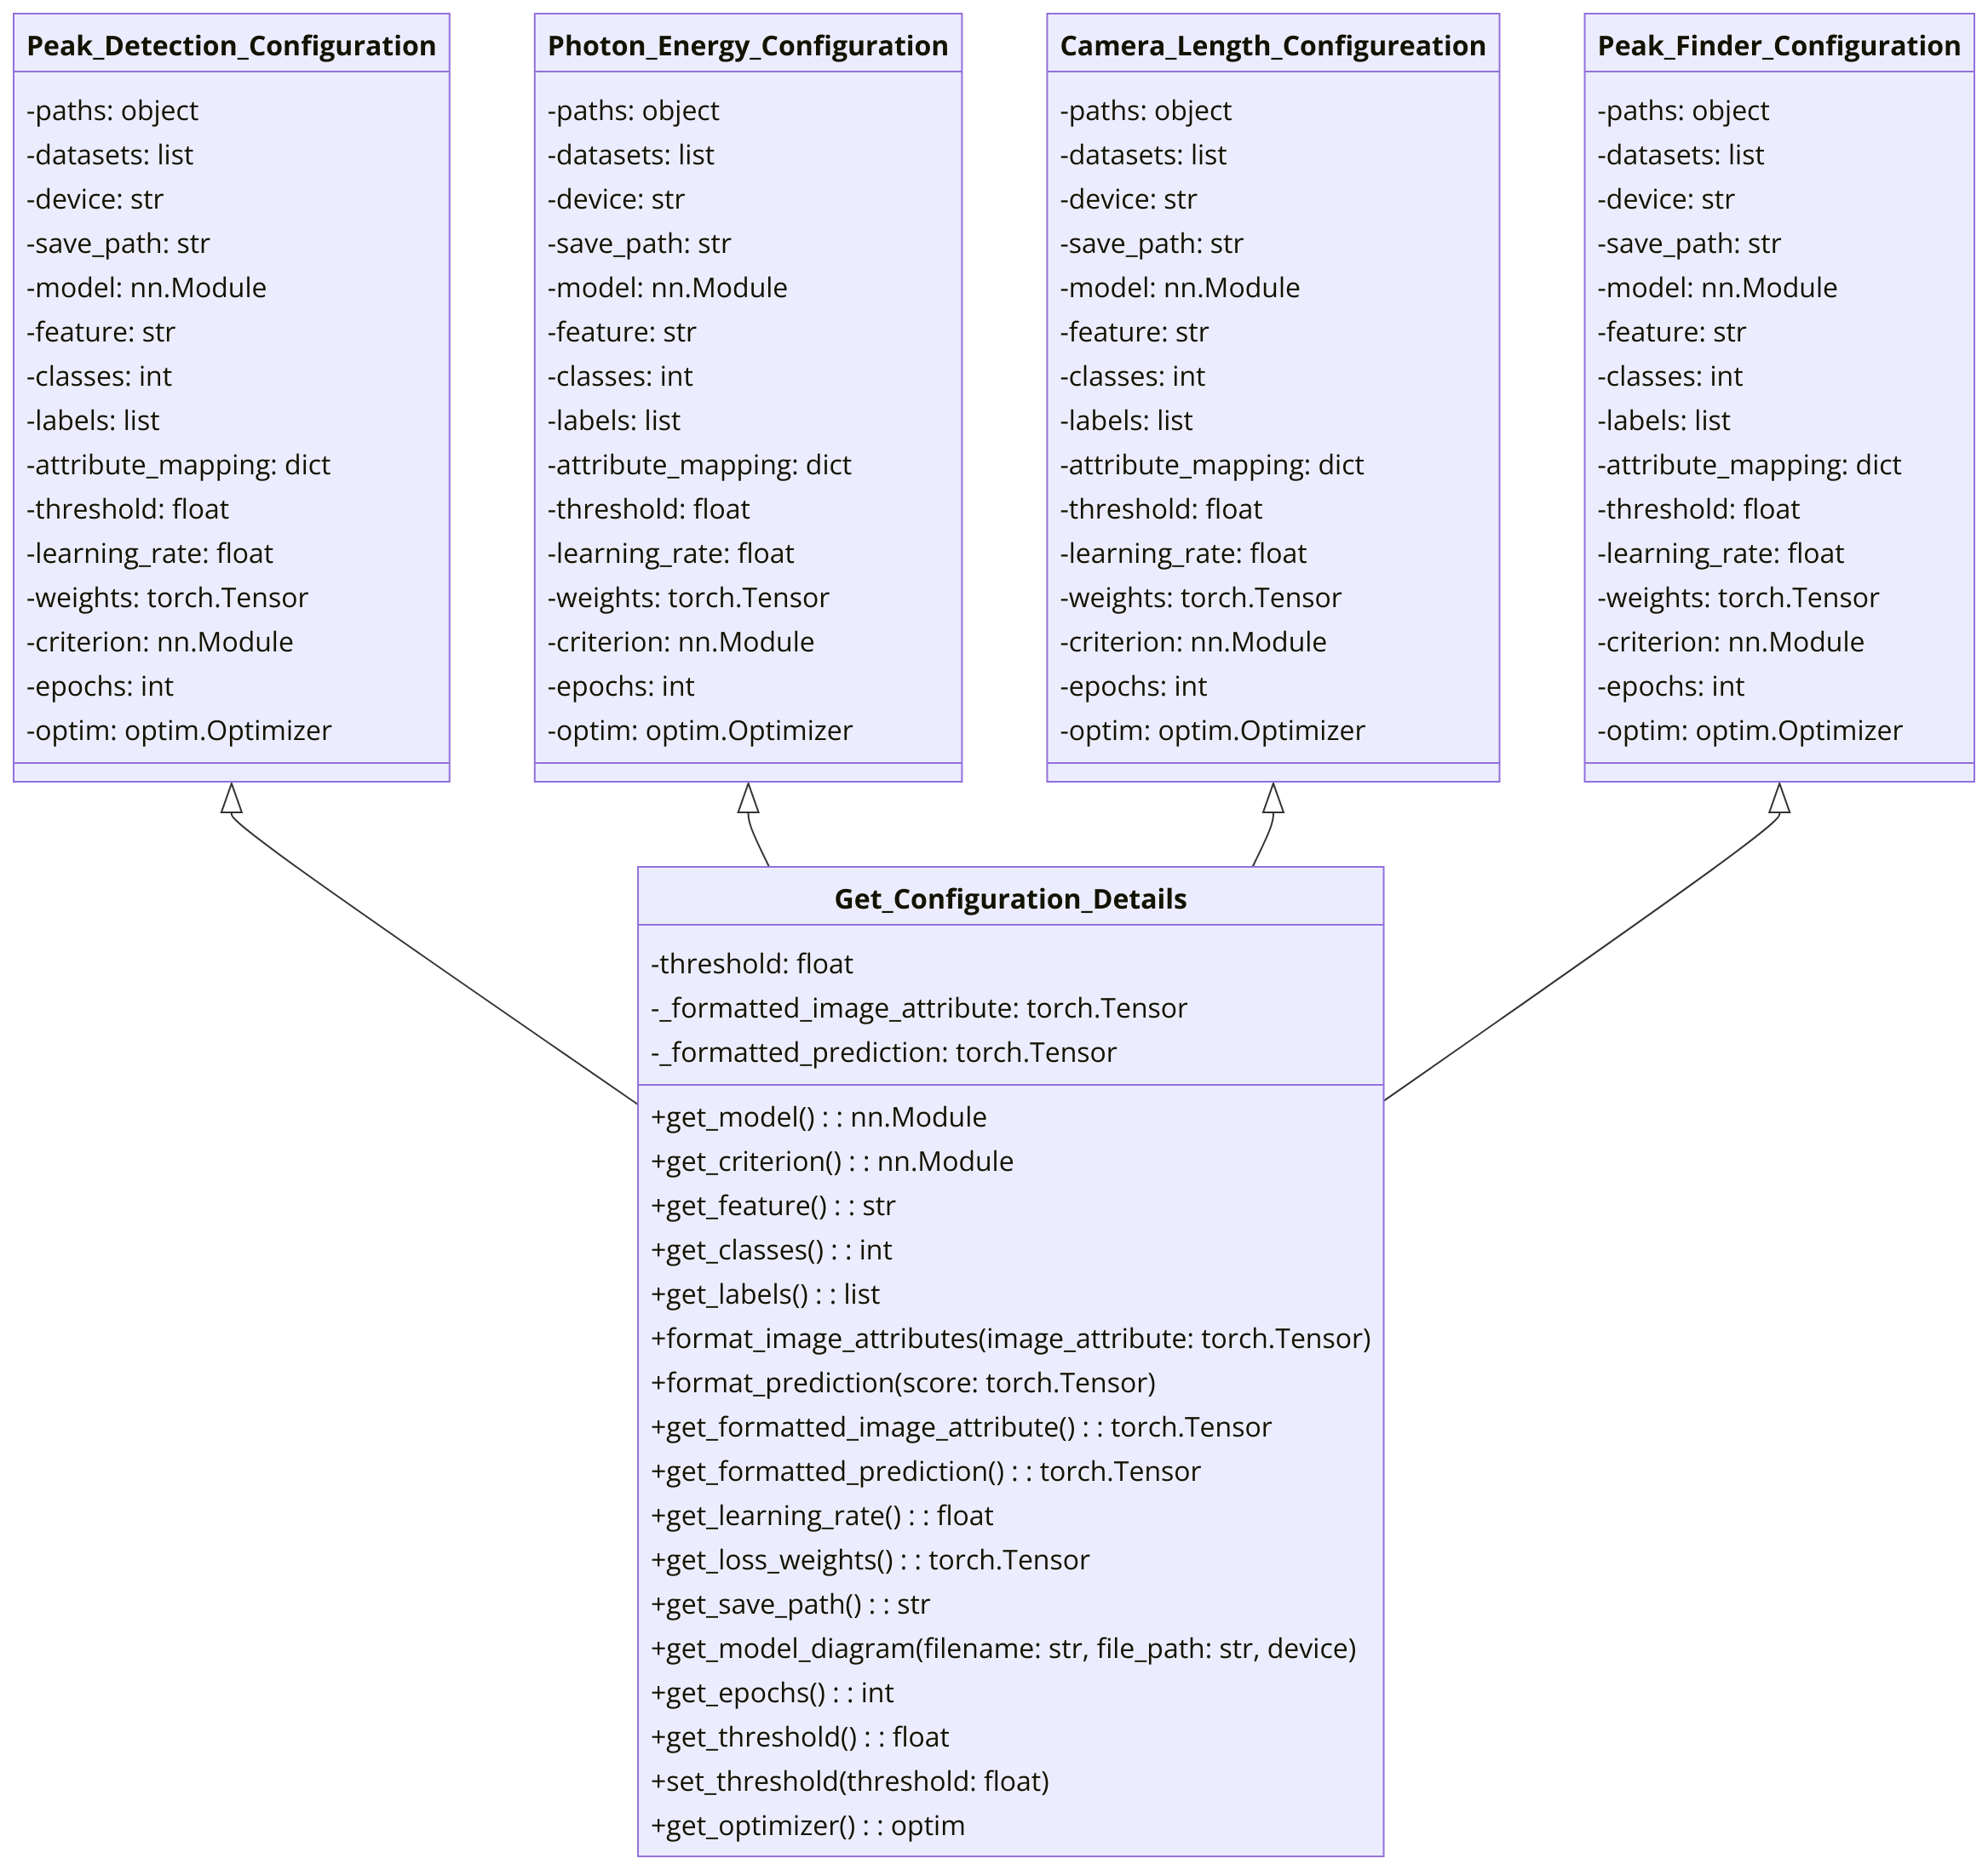
\includegraphics[width=0.6\textwidth]{uml_diagrams/eval_uml2.png}
    \caption{eval.py UML diagram}
    \label{fig:eval}
\end{figure}

The first model, as seen in Figure~\ref{fig:binary_model} is the first in the pipeline. This being a CNN designed for binary classification; this being peak detection. However, this was by far the most difficult model to get adequate results from due to the low flux nature of the CXLS data. The Bragg peak detection was a very difficult due the closeness in value of the signal and noise. This is why the novel approach we introduce is necessary. Figure~\ref{fig:binary_model} highlights the two convolutional layers optimized for extracting varying scales of features from images. The first convolutional layer uses a larger \(10\times10\) kernel to capture broad features, followed by a smaller \(3\times3\) kernel in the second layer for finer details. Each convolutional layer incorporates group normalization with four groups to ensure stable and efficient training by normalizing group activations. After the initial convolutional layer, a max pooling step reduces the spatial dimensions by half, which decreases the computational load and helps mitigate overfitting. The network utilizes the ReLU activation function after each group normalization to introduce non-linearity, enhancing the model's ability to learn intricate patterns. The output from the convolutional layers is dynamically computed to ensure accurate dimensionality for flattening before it reaches the fully connected layer. This layer is crucial as it integrates all the learned features to make the final classification decision. The model's dynamic architecture, including calculated output dimensions and the subsequent flattening of these dimensions, enables efficient processing and robust performance in classifying complex image data.\\

For binary classification peak detection, It was found that implementing a learning rate scheduler helped the problem converge on a solution faster. The scheduler used is ReduceLROnPlateau. The parameters we used where reducing the learning rate by a factor of 10 every 3 epochs there was not a change in the learning rate at a threshold of 0.1. It was also found that using weights was beneficial to the peak detection problem. This is likely because we are generating empty images based of a percent of the simulated data. Therefore, weights would be helpful due to the imbalanced nature of the dataset. The weight used for binary classification was calculated by dividing the total number of empty images by the number of peak overlay images, giving a weight of about 0.4. The loss function used for binary classification was BCEWithLogits which combines the sigmoid activation function with binary cross entropy. This loss function is very numerically stable and computationally effective. The optimizer used for binary classification is Adam. This optimizer is computationally expensive compared to other optimizers, like stochastic gradient descent, but outcome from using Adam was always superior and thus warranted incorporation.\\

\begin{figure}[H]
    \centering
    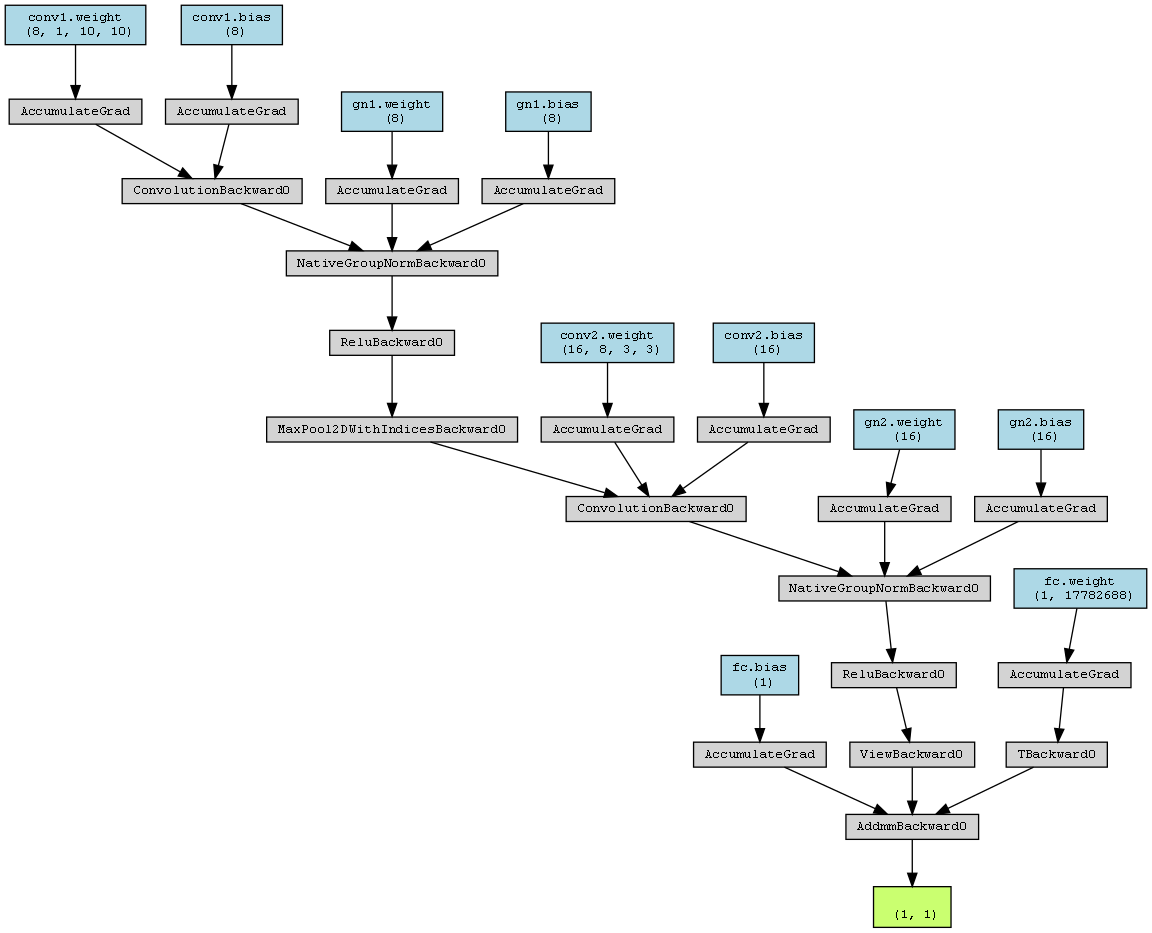
\includegraphics[width=0.75\textwidth]{models/peak_binary_model.png.png}
    \caption{Peak binary classification model made by torchviz.}
    \label{fig:binary_model}
\end{figure}

To increase the complexity of the binary classification problem in a realistic way, we used data were the beam size was not optimized to the sample protein, causing many of the photons to miss the target, lowering the flux even more. Interestingly, we got the best results not by adding more layers to increase complexity, but by using the next model, dual input CNN, where it would train with both overlay images and signal images.\\

The next model, seen in Figure~\ref{fig:dual_model}, uses two separate but identical branches. Each branch consists of a convolutional layer with a \(5\times5\) kernel, a stride of 2, and padding of 1, followed by a ReLU activation and a max pooling layer. This design helps in extracting and reducing feature dimensions effectively for both overlay and respective peak images. Output dimensions from both branches are calculated dynamically to ensure consistency before the features are flattened and concatenated. This combined feature set is then fed into a classifier that includes a linear layer with 128 units, a ReLU activation, and a final linear layer that outputs a single decision value. Like for the normal flux classification, we used BCEwithLogits, Adam, and ReduceLROnPlateau.\\

\begin{figure}[H]
    \centering
    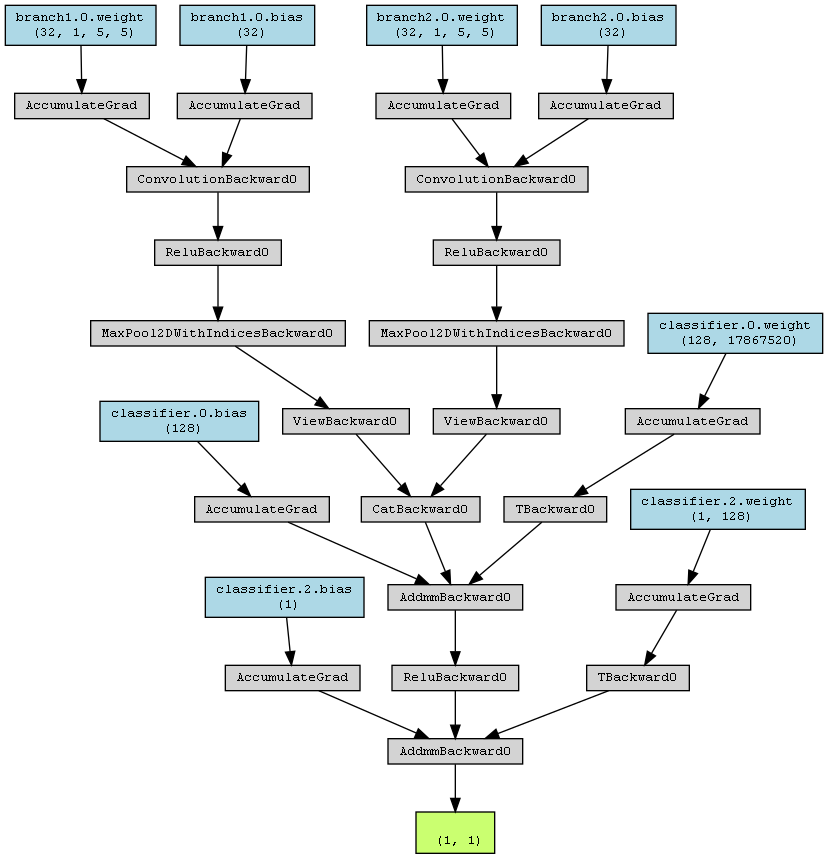
\includegraphics[width=0.5\textwidth]{models/peak_detection_model.png.png}
    \caption{Model of dual input CNN.}
    \label{fig:dual_model}
\end{figure}

The photon energy and camera length are both multi-class classification problems with three output classes for each. The camera length and photon energy effect the overlay and peak images so much that this is a problem that could be addressed with just a linear model. We used stochastic gradient descent (SGD) for these models because they would produce the same results with less computational cost than Adam, and there was no need for a learning rate scheduler. For the loss function, we used cross entropy loss.\\

The state dictionaries for the models for peak detection (normal flux), photon energy classification, and camera length classification were saved after training. These saved parameters would then be used in the model pipeline. This pipeline is created by instantiating the pipeline class from \texttt{pipe.py} and passing in the attribute objects and file paths to the saved parameters. We then would use the \texttt{run} function, which takes in an image tensor, and send it through the binary classifier. If peaks were detected, then the image would then be passed to the other multi-class classifiers, for the prediction of camera length and photon energy. At the end of this pipeline, the output value would either be false, ending in termination after peak detection, or return true with the camera length and photon energy predictions. This serves as a prototype for what the final product will act like when being used for the CXLS.\\

\begin{figure}[H]
    \centering
    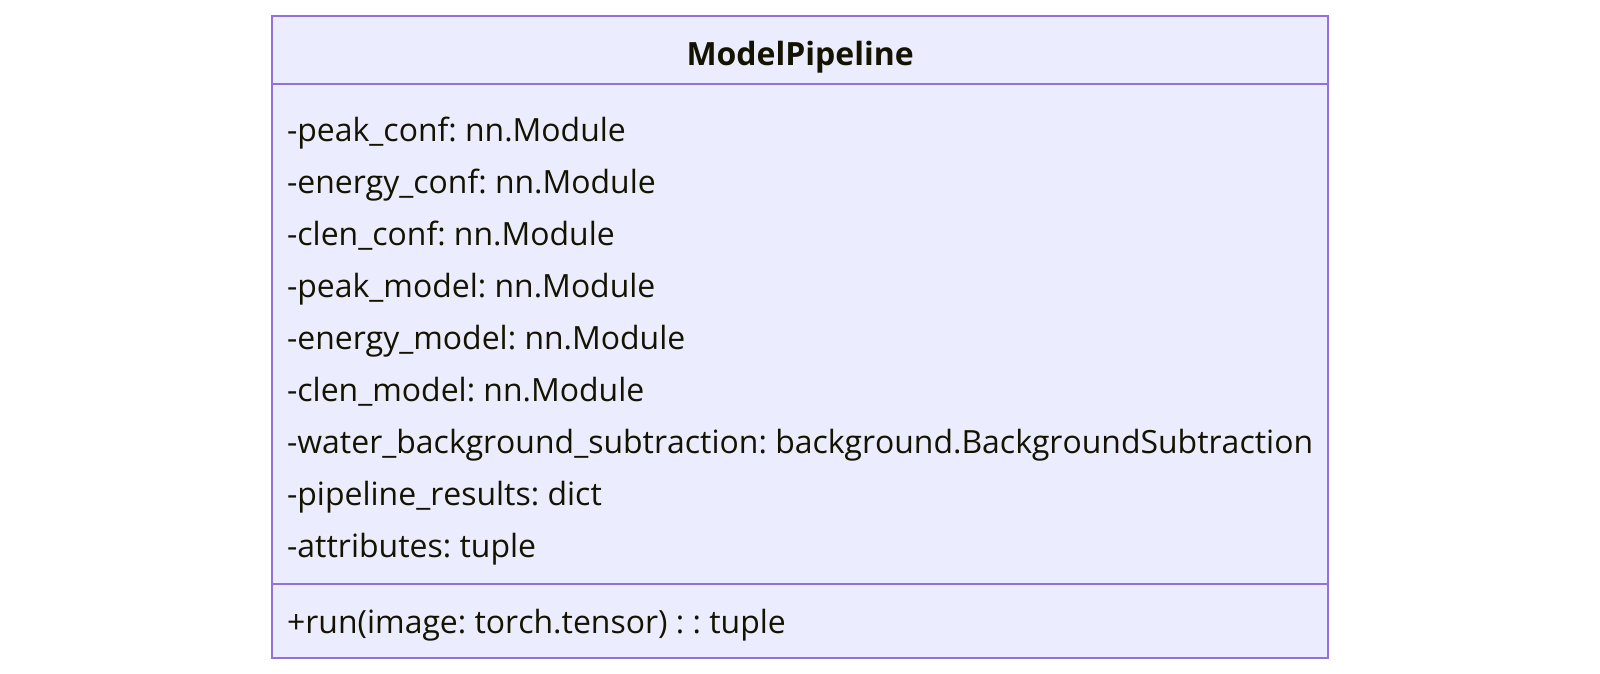
\includegraphics[width=0.75\textwidth]{uml_diagrams/pipe_uml.png}
    \caption{pipe.py UML diagram}
    \label{fig:pipe}
\end{figure}

The last model we worked on was a model for finding peak locations. This model is by far the most complex model, seen in Figure~\ref{fig:peak_finder}. This model is mentioned after the pipeline because it is not to a satisfactory level yet, and therefore excluded from the pipeline.\\

This model is a convolutional neural network designed to generate heatmaps from image inputs. It starts with an initial convolutional layer that expands the input to 16 channels, followed by batch normalization and a max pooling layer to reduce dimensionality. A second convolutional layer increases the channel depth to 32, followed by another batch normalization. The network then incorporates advanced attention mechanisms to refine the feature maps; ChannelAttention, which focuses on important features across the channel dimension by processing average and max pooled signals through separate fully connected layers, and SpatialAttention, which focuses on critical spatial information by processing the maximum and average projections of the feature maps.\\

These attention mechanisms enhance the network's ability to focus on relevant features, both channel-wise and spatially, allowing for more precise heatmap generation. After processing through these attention modules, the feature map is passed through another convolutional layer specifically designed to produce the heatmap output. Finally, the heatmap is upscaled to the original input size using bilinear interpolation and a dropout layer is applied to prevent overfitting.\\

\begin{figure}[H]
    \centering
    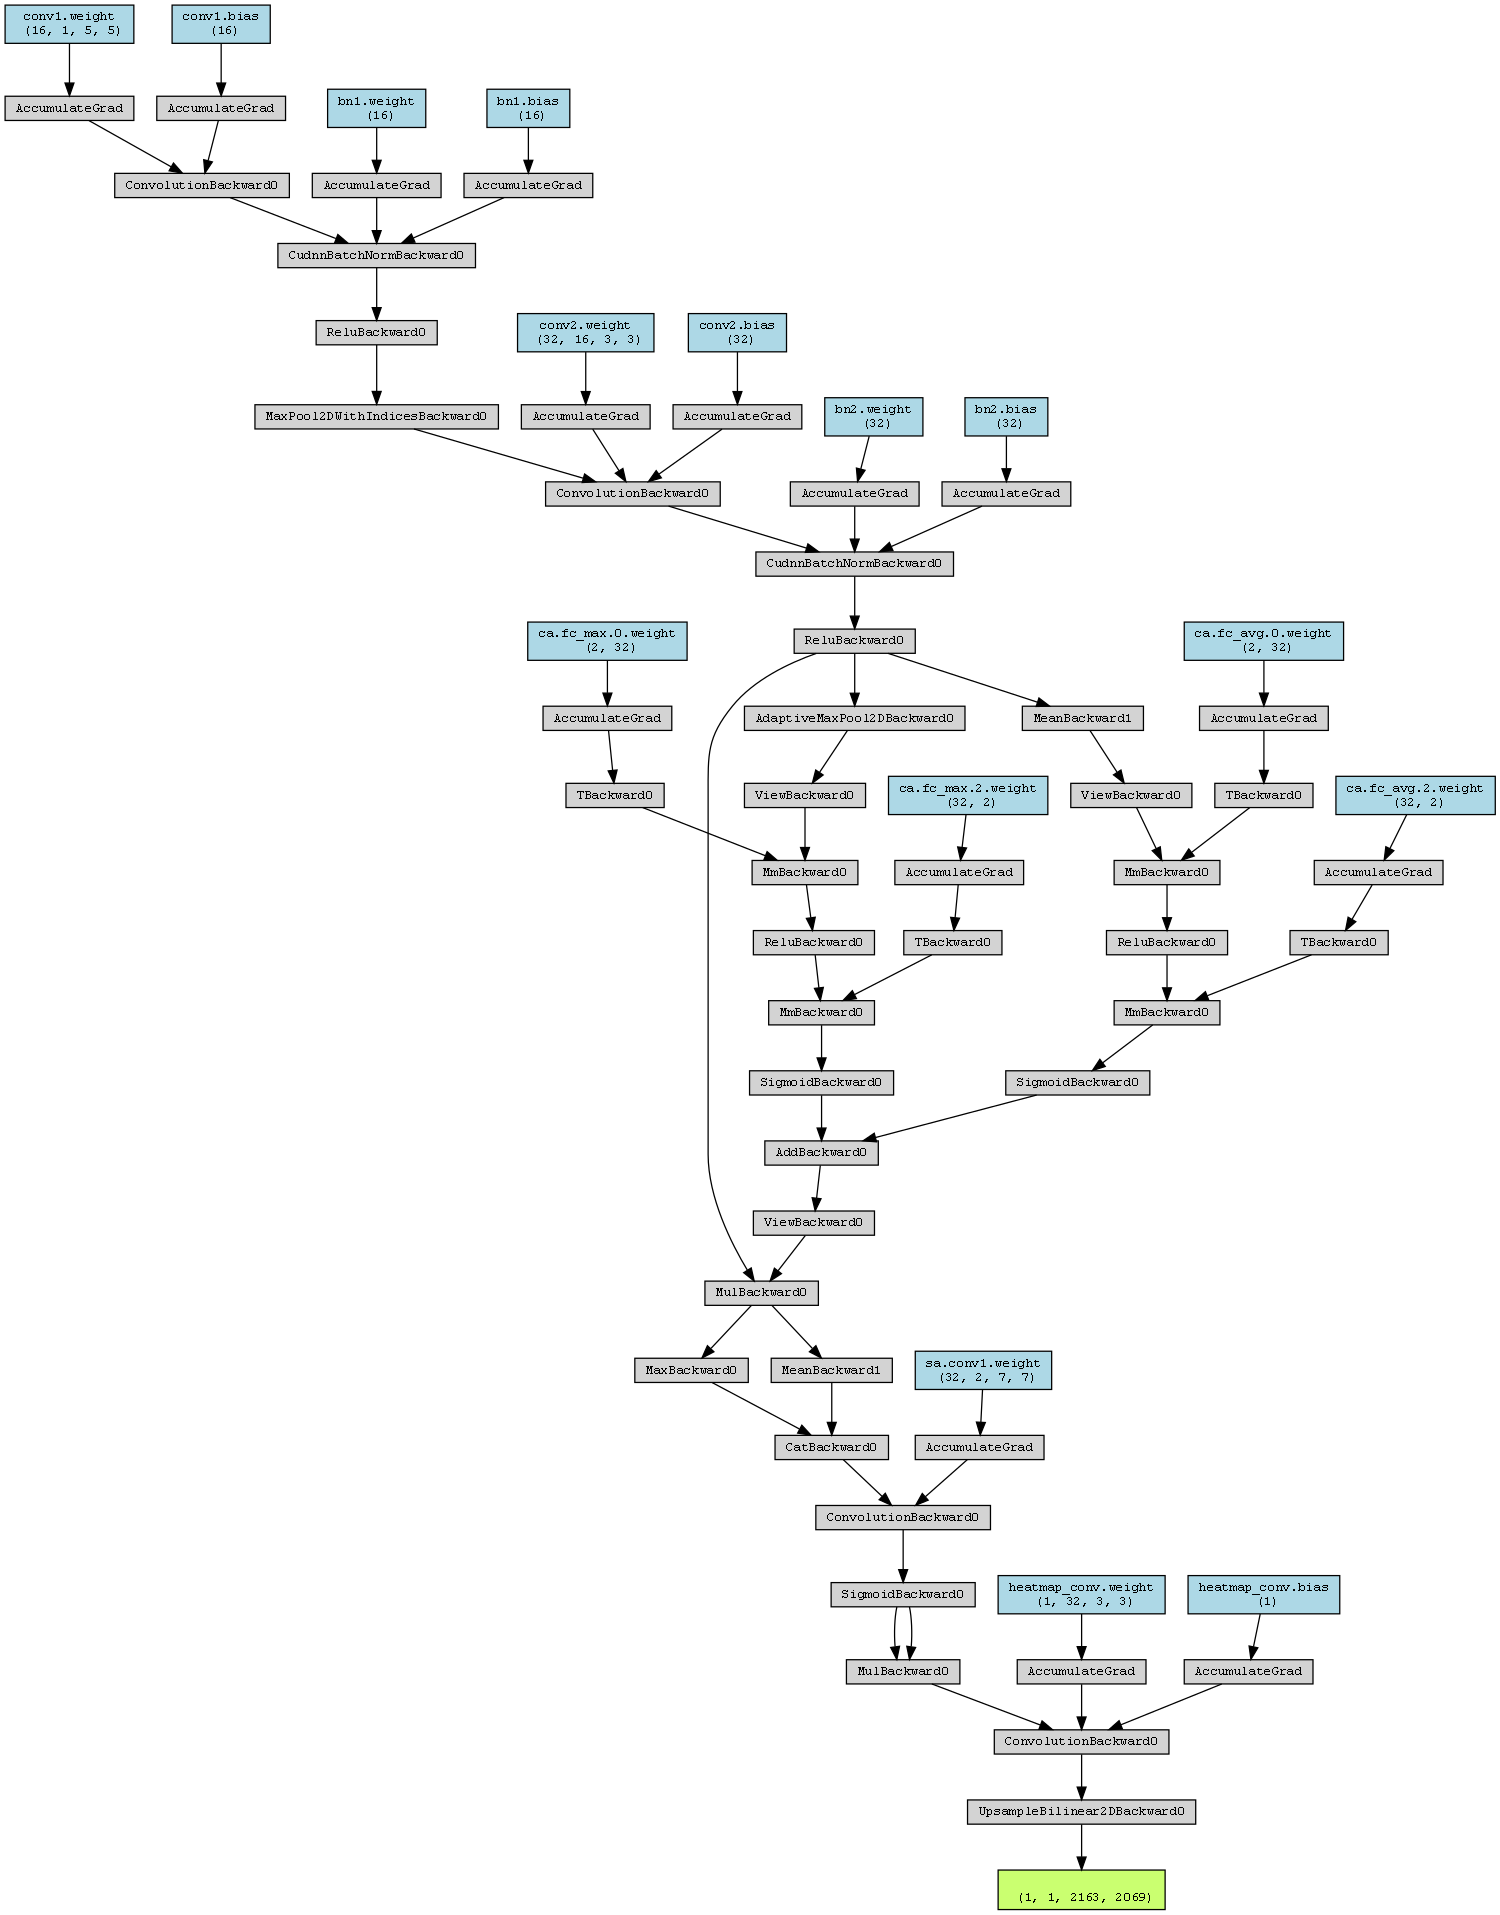
\includegraphics[width=0.75\textwidth]{models/first_peak_finder_model.png.png}
    \caption{Current status of the peak finder model.}
    \label{fig:peak_finder}
\end{figure}

\section{Results}

The results for both photon energy and camera length classification resulted in a model that could perfectly classify the images. Each model produced a confusion matrix of diagonal ones. As well, by the end of the fifth epoch on each model the train and test accuracy was one and the train and test loss was zero. We can even see in Figure \ref{fig:photon_energy_example} that if we change the data sets being used in training that the model will appropriately respond.\\

\begin{figure}[H]
    \centering
    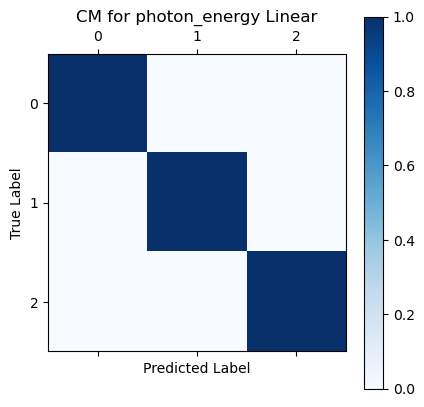
\includegraphics[width=0.4\textwidth]{confusion_matrix/photon_cm.png}
    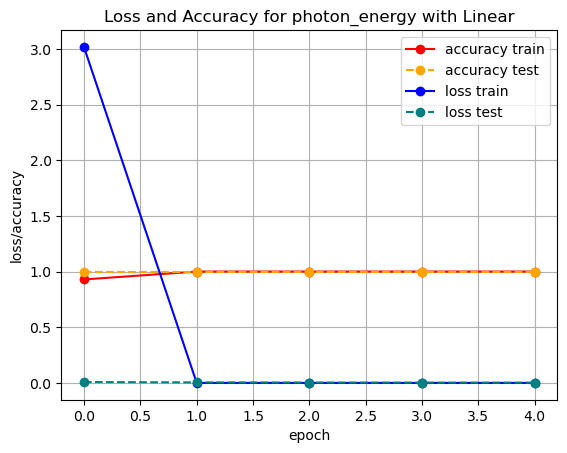
\includegraphics[width=0.4\textwidth]{loss_plot/photon_loss.png}
    \caption{Results from training the linear model for classifying photon energy.}
    \label{fig:photon_energy_results}
\end{figure}

\begin{figure}[H]
    \centering
    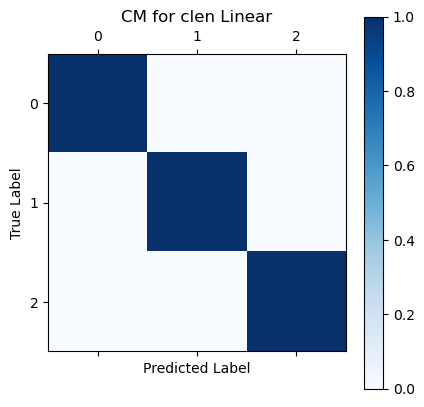
\includegraphics[width=0.4\textwidth]{confusion_matrix/camera_cm.png}
    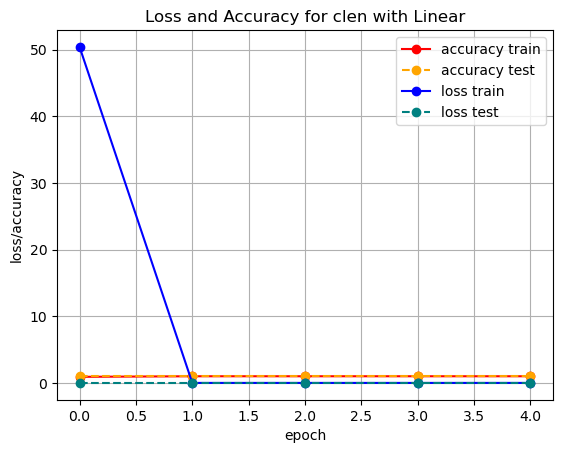
\includegraphics[width=0.4\textwidth]{loss_plot/camera_loss.png}
    \caption{Results from training the linear model for classifying camera length.}
    \label{fig:photon_energy_results}
\end{figure}

\begin{figure}[H]
    \centering
    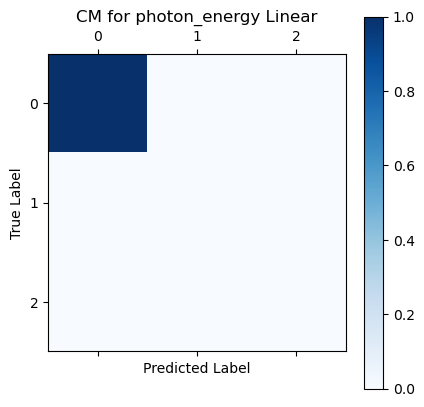
\includegraphics[width=0.5\textwidth]{confusion_matrix/photon_energy_example_cm.png}
    \caption{This is an example of selecting specific data sets, here \texttt{01} and \texttt{02}, and seeing that the model properly classifies the data.}
    \label{fig:photon_energy_example}
\end{figure}

Below is the training for the normal flux binary classification, which was almost perfect. With 30 epochs, the final confusion matrix came out to be,

\[
    \begin{bmatrix}
        1 & 0\\
        0.025 & 0.975\\
    \end{bmatrix}
\]

\begin{figure}[H]
    \centering
    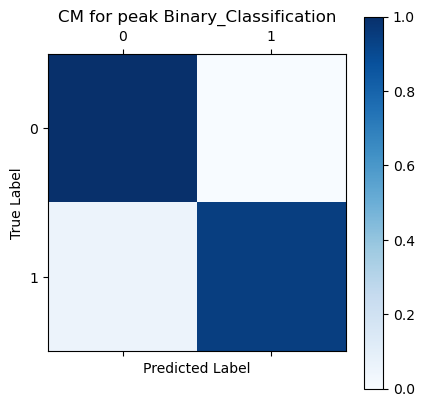
\includegraphics[width=0.4\textwidth]{confusion_matrix/binary_cm.png}
    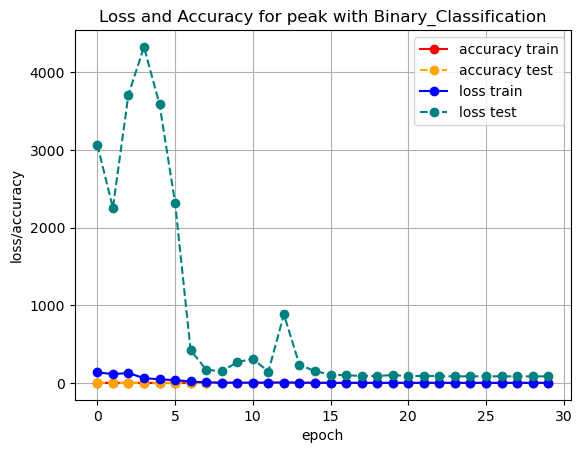
\includegraphics[width=0.4\textwidth]{loss_plot/binary_loss.png}
    \caption{Results from training binary model for classifying normal flux photon peaks.}
    \label{fig:binary}
\end{figure}

Below is the comparison base CNN used to justify a more complex architecture. The base CNN is composed of a convolutional layer, the ReLu activation function, and a fully connected layer. Over the same number of epochs, the outcome confusion matrix was 
\[
\begin{bmatrix}
    1 & 0 \\ 
    0.26 & 0.74\\
\end{bmatrix}
\]

The improvement on peak detection here is critical, as misidentifying 26\% of peak data would be detrimental in data analysis. Thus warranting the basic CNN as not suited for our purposes. \\

\begin{figure}[H]
    \centering
    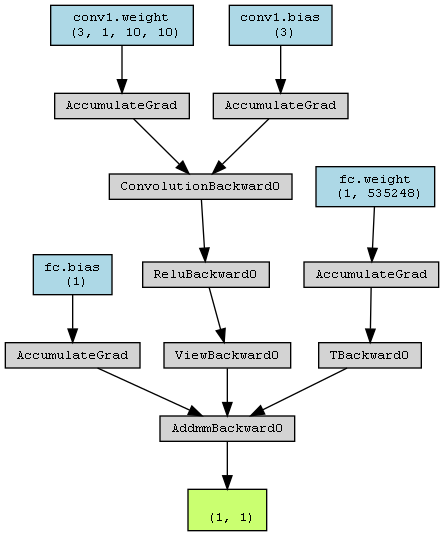
\includegraphics[width=0.4\textwidth]{models/peak_base_model.png.png}
    \caption{This is the base binary classification model used to comparison made by torchviz.}
    \label{fig:base_model}
\end{figure}

\begin{figure}[H]
    \centering
    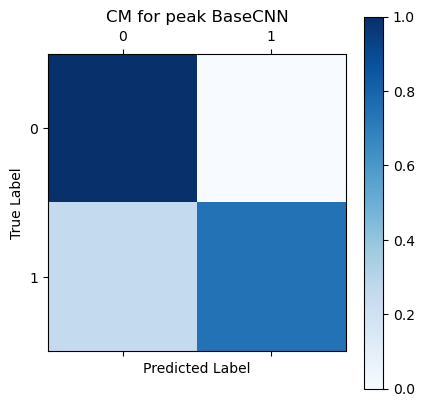
\includegraphics[width=0.4\textwidth]{confusion_matrix/binary_base_cm.png}
    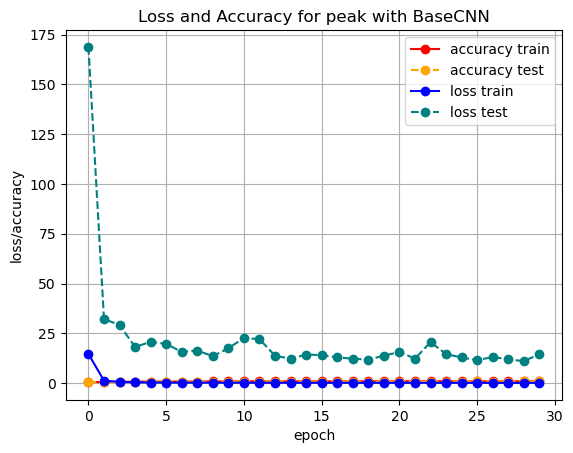
\includegraphics[width=0.4\textwidth]{loss_plot/binary_base_loss.png}
    \caption{Base comparison model for binary classification.}
    \label{fig:binary_base}
\end{figure}

Using the train models, we loaded that \texttt{state\_dict} of the models from their respective pt files into the ModelPipeline class. We passed in diffraction images into the run method and it classified the image. Below in Figure~\ref{fig:pipeline_true} are examples of classification of images with and without Bragg peaks.\\

\begin{figure}[H]
    \centering
    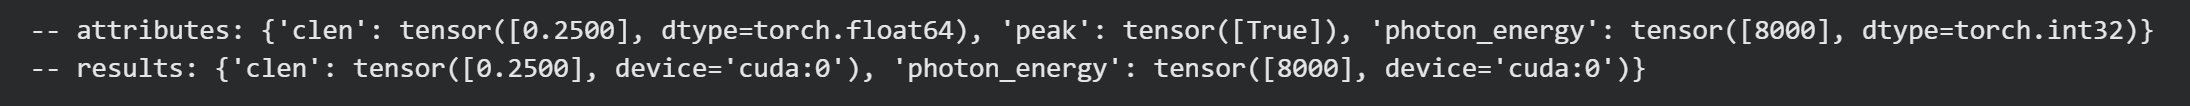
\includegraphics[width=1\textwidth]{pipeline_true.png}
    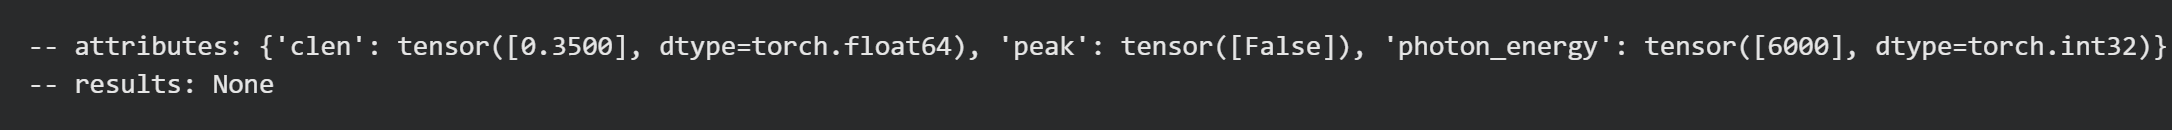
\includegraphics[width=1\textwidth]{pipeline_false.png}
    \caption{Example pipeline results.}
    \label{fig:pipeline_true}
\end{figure}

Below are the results from the extreme low flux from the beam misalignment. These parameters caused classification to be very difficult for the model, producing a confusion matrix of 

\[
\begin{bmatrix}
    0.25 & 0.75\\
    0 & 1\\
\end{bmatrix}
\]

While the loss and accuracy plot do not show this, the loss and accuracy would plateau for up to 30 epochs, when with the use of a learning rate scheduler. Despite being difficult to classify, this is the only model that would not result in complete classification of either "peaks" or "no peaks" (columns in the confusion matrix). Even the model used for normal flux peak detection was producing poor results with this data set in Figure~\ref{fig:dual}.\\

\begin{figure}[H]
    \centering
    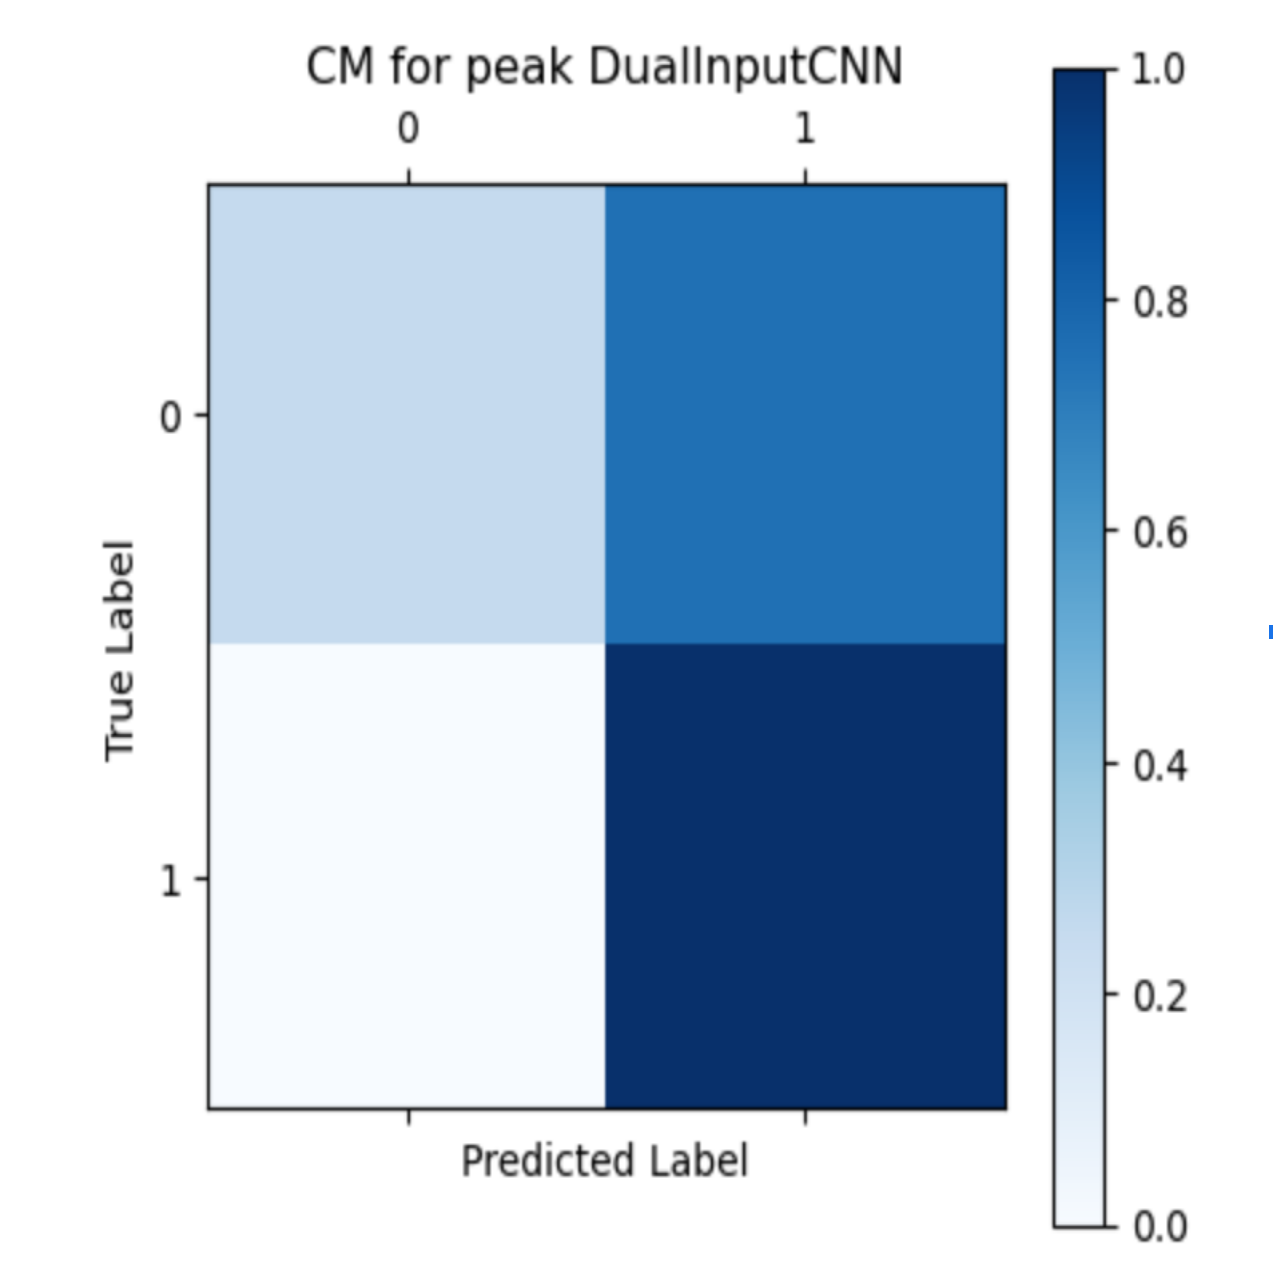
\includegraphics[width=0.4\textwidth]{confusion_matrix/dual_cm.png}
    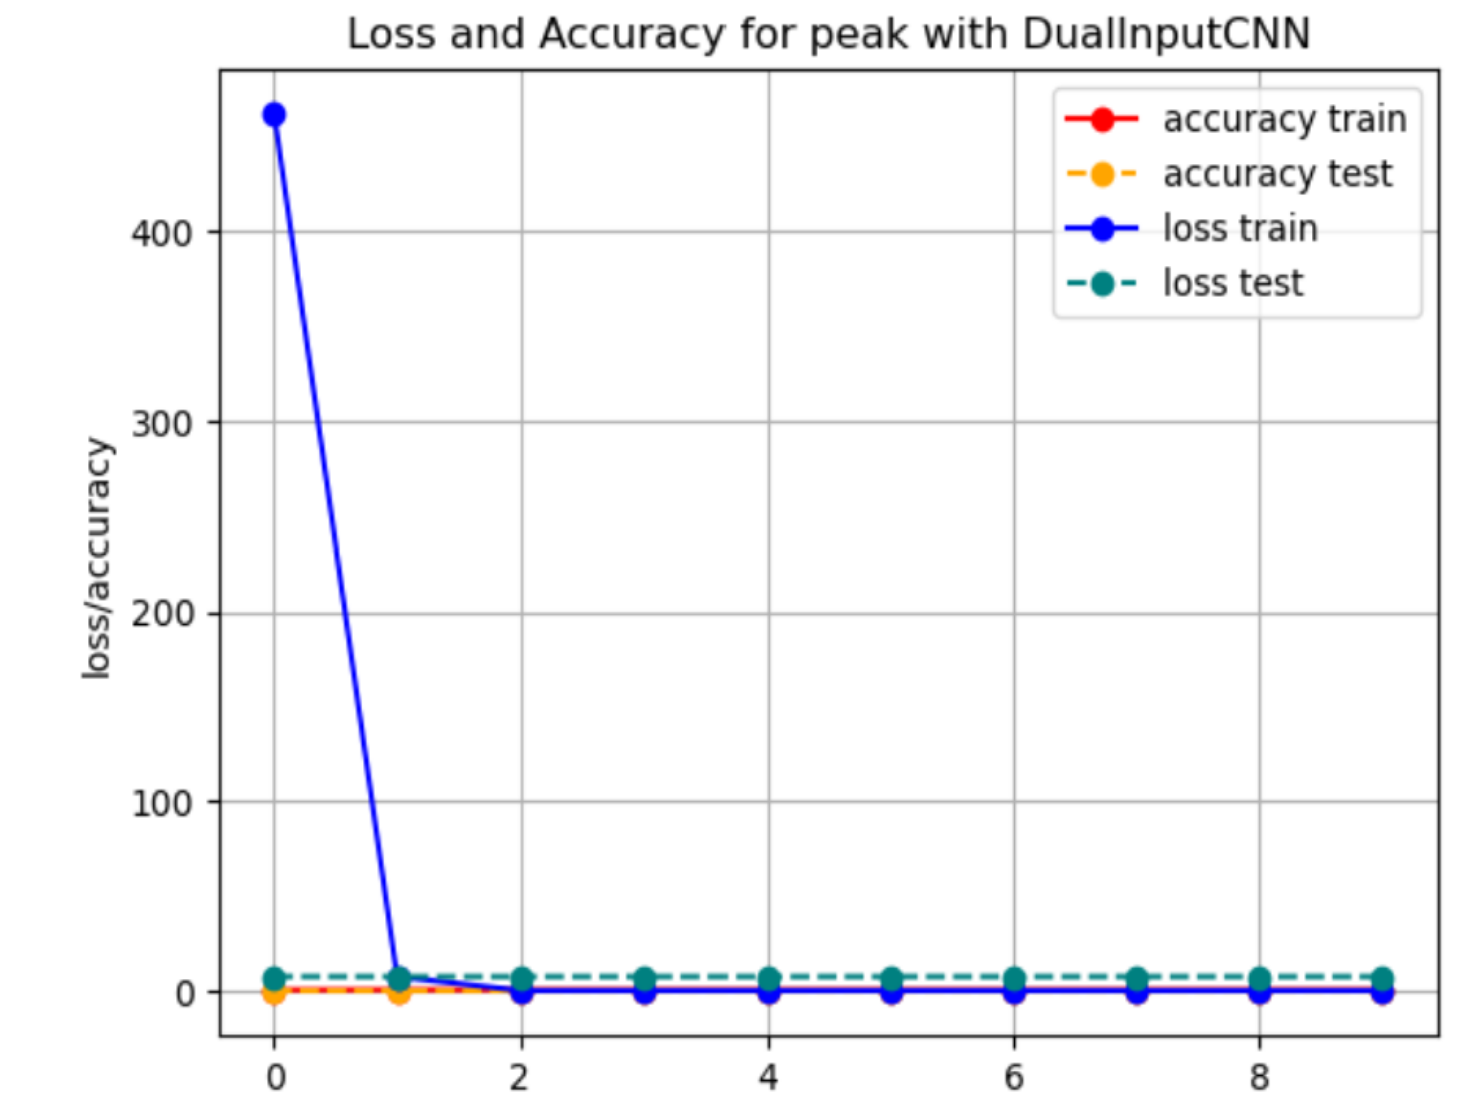
\includegraphics[width=0.4\textwidth]{loss_plot/dual_loss.png}
    \caption{Results from training dual channel model for classifying extreme low flux photon peaks.}
    \label{fig:dual}
\end{figure}

In Figure~\ref{fig:peak_finder} is the results from the peak finder model. The loss and accuracy graph is deceiving in this situation. Since our diffraction images have over 4 million pixels (roughly \(2000 \times 2000\)), and there is about 1 peak pixel per 100,000 noisy pixels, the low loss and high accuracy does not accurately give a good representation of how to model doing in reality. The confusion matrix does however show that the model is over fitting to give that there are never Bragg peaks.\\

\begin{figure}[H]
    \centering
    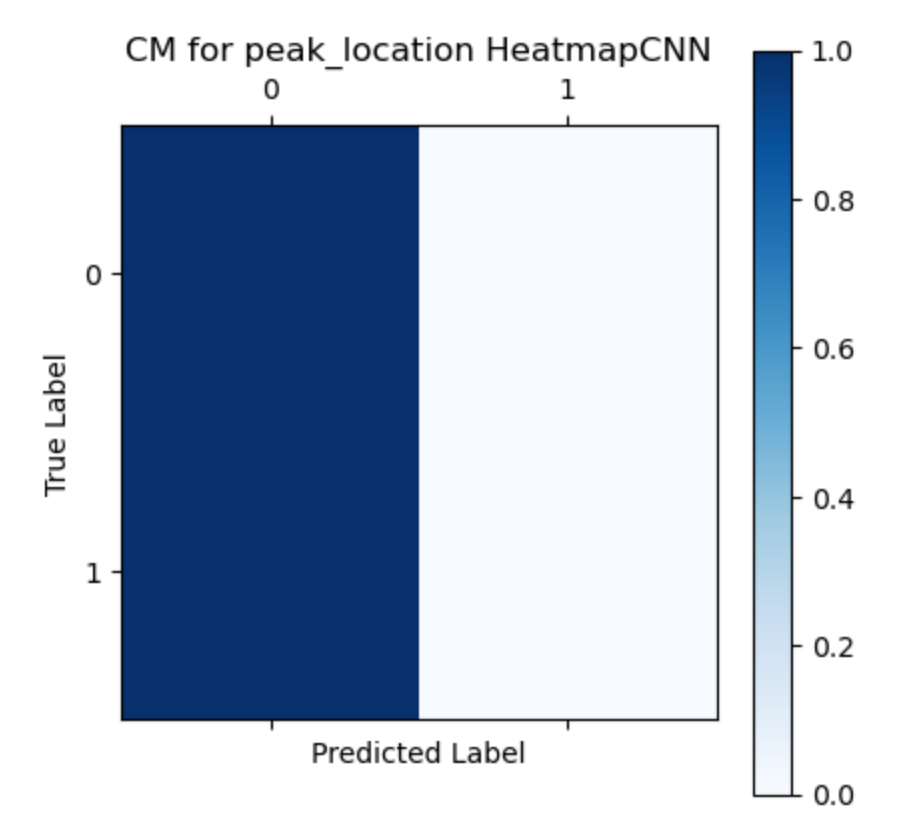
\includegraphics[width=0.4\textwidth]{confusion_matrix/peak_finder_cm.png}
    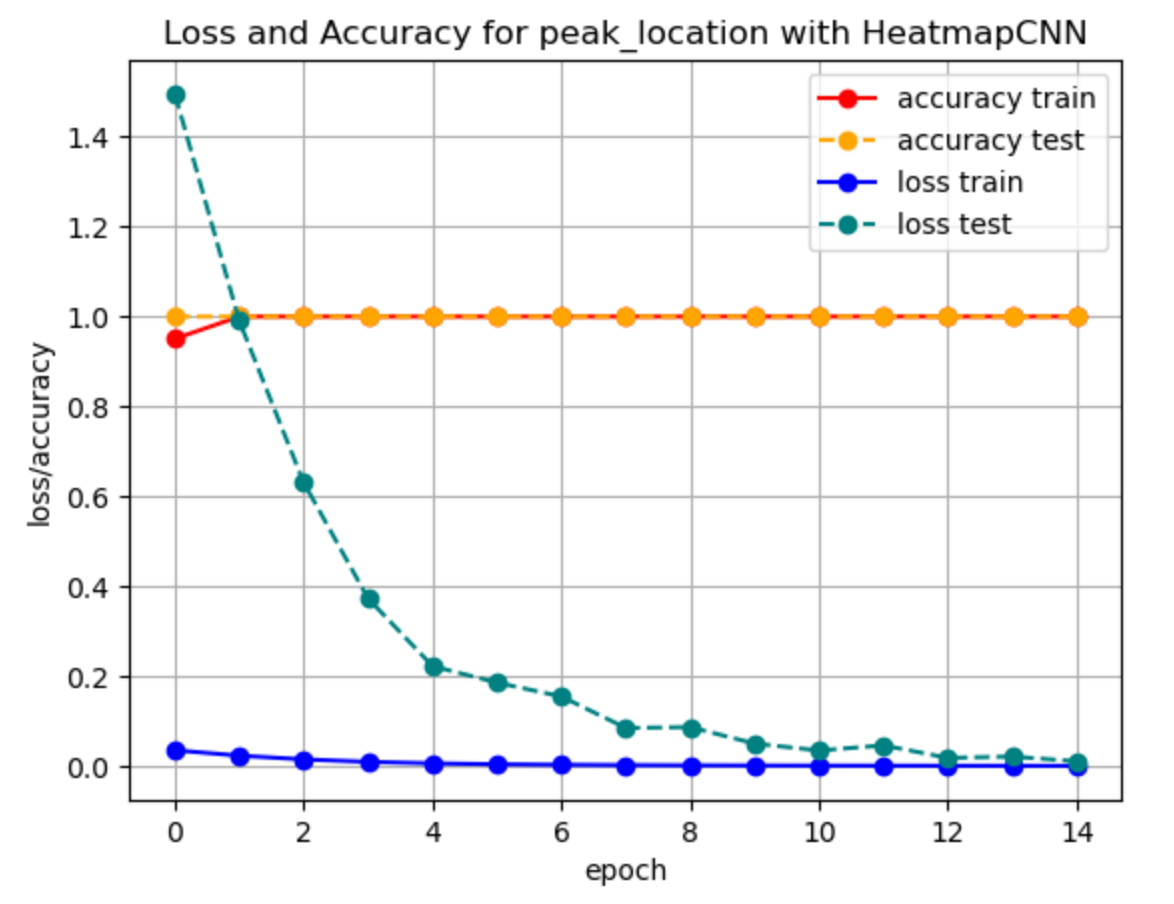
\includegraphics[width=0.4\textwidth]{loss_plot/peak_finder_loss.png}
    \caption{Results from training peak finder model.}
    \label{fig:peak_finder}
\end{figure}


\section{Discussion}

The multi-class classification problems with our parameters ended up being much simpler to classify that previously imaged. We started working with CNNs for this classification and realized that all that was needed was a linear model. This is likely the case because of the values and amount of chosen photon energies and camera lengths to work with. If we had a larger spectrum of photon energies and camera lengths it would likely be much more difficult to classify. The next step in expanding the capabilities of this model now that we know this is an easy task is to generate more data categories, which was too time consuming to reasonably do within the time frame of this project. Ideally we would be able to classify to the nearest keV photon energy and nearest cm camera length.\\

The binary classification with normal flux was difficult to accomplish because it was mostly in tuning parameters. Creating models with more layers would still only result in less than 75\% of correctly identified peak images. We  found after creating multiple models and playing with the parameters that the model we choose gave the best results for the lest computational cost. The accuracy seems to plateau at around 95\% accuracy for detecting peaks, even with more epochs. This may come down to fine tuning the model even more.\\

Binary classification for extreme-low flux was incredibly difficult to figure out. Even using methods like transfer learning with models architectures like ResNet50 could not produce results as good as the dual channel input. We also attempted single channel input with both peak and overlay images for training, and testing with only overlay, however this lead to poor results as well. Of course the glaring issue with this implementation would be using this model in a practical sense, due to a channel requiring the need of a signal image. This will need to be explored more because while the lab does not expect to see images this low flux commonly, it would be better if our model could handle a variety of photon fluxes.\\

The peak detection model was severely over fitting the data to always give the results that there is no Bragg peaks. Even when incorporating a high weight of 100,000 for the loss function, and using a high dropout rate of 0.9, the model eventually starts to guess all zeros over enough epochs. The model also seems to never get any peak identification location correct. We were able to monitor this by watching a printout of the known and guessed peaks. The model seems to learn before 10 epochs that there are only around 10 to 100 peaks present in the image, and it also seems to start to group the guessed peaks in the correct areas. However, it never actually guesses a peak correctly, it over fits before that can happen. We have also played with using a DnCNN (denoising convolutional neural network), however the results of this model did not seem to work as well. This will be the main focus of this project after this class ends. Being able to local the peaks is long term the heart of this project, and will likely be the first thing we tackle during the summer at CXFEL Labs.\\

In this project data simulation and management was a bottleneck. It was a slow start to get software running for data simulation, and it was a long stretch to get all the correct data we needed. We spent quite some time working with incorrect data until we were able to clear the issues with our P.I. at CXFEL Labs, which lead to us experimenting with the extreme low flux data, since it was already generated. Though this low flux data was not meant to be used at this point, it lead to interesting results for a real issue that was not originally part of this project, but worth mentioning in the report. Issues with file management code would stop the ability to test models for days at a time while troubleshooting. Now that these prospects are in order, we are currently simulating thousands of images to use to use with training, and the file management code is incredibly robust and easy to troubleshoot.\\

In conclusion, this project has significantly advanced the understanding and application of deep learning techniques in the analysis of X-ray crystallography data for the CXLS at ASU. By successfully integrating CNNs, we have enhanced the accuracy and efficiency of peak detection and the prediction of experimental parameters, demonstrating the potential of advanced computational methods in overcoming the inherent challenges posed by low flux and high noise levels in diffraction data. This research not only serves as a foundational study in applying neural networks to crystallography at CXLS but also sets the stage for future work to expand these techniques to include more complex experimental setups and broader applications in scientific research. Moving forward, it is anticipated that continued refinement of these models and expansion of the data set will yield even more robust tools, capable of transforming the landscape of crystallographic research by significantly reducing the time and resources needed for data analysis.\\

% Bibliography setup
\bibliographystyle{plain} % This defines the style of the bibliography
\bibliography{references} % This points to the file containing the BibTeX entries


\end{document} 

